\apendice{Especificación de diseño}

\section{Introducción}

En este apéndice se recogen las características de diseño que implementan los requisitos descritos en el apéndice anterior, a fin de establecer los criterios que se deberán seguir en el desarrollo del sistema.

\section{Elección del nombre del proyecto}

Para la elección del nombre bajo el cual se englobara todo el servicio de resumen de textos en la nube, se consideraron numerosas opciones, de las cuales, las más relevantes fueron:

\vspace{-0.2cm}
\begin{itemize} [\textbullet]
	\item \textbf{Summit}: acrónimo procedente de \emph{Summarize it}. Además, <<\emph{summit}>> tiene el significado de <<cumbre>> o <<cima>> en inglés, sugiriendo el alto rendimiento y potencia del servicio, alcanzando los más \emph{altos} resultados.
	
	\item \textbf{Jizt}: esta palabra, pronunciada en inglés, suena casi idénticamente a <<\emph{gist}>>, la cual se puede traducir como <<esencia>> o <<quid de la cuestión>>.
	
	\item \textbf{Halb}: al revés se lee <<\emph{blah}>> (de \emph{blah, blah, blah}, en inglés) y en alemán significa <<mitad>>, evocando a la idea de resumen. Además se podría ver como una referencia al supercomputador HAL 9000 de la película y posterior novela \emph{2001: Una Odisea del Espacio}.
\end{itemize}

De estas tres, se juzgaron más interesantes las dos últimas; la primera resulta menos original debido a que ya existen numerosas empresas, productos y proyectos con este nombre.

En ese momento, se llevó a cabo una pequeña encuesta para determinar el nombre final. Dado que el proyecto aspira a tener un carácter internacional, el objetivo de la encuesta no era tanto obtener un gran numero de votaciones, sino que las que tuviéramos fueran muy variada: en total se preguntó a 22 personas de 15 nacionalidades diferentes.

A continuación, se incluye una tabla resumiendo los resultados de la encuesta:

\vspace{0.5cm}
\begin{table}[h]
	\centering
	\begin{tabular}{>{\raggedright}b{0.168\textwidth}>{\centering}b{0.2\textwidth}>{\centering\arraybackslash}b{0.2\textwidth}}
		\toprule
		\multicolumn{3}{c}{\large\textbf{Elección de Nombre}} \\
		\smallskip
		& \textbf{\emph{jizt}} & \textbf{\emph{halb}} \\
		\midrule
		\small{España} & \small{2} & \small{3} \\
		\small{Alemania} & \small{3} & \small{0} \\
		\small{México} & \small{1} & \small{1} \\
		\small{Taiwán} & \small{1} & \small{0} \\
		\small{Japón} & \small{0} & \small{1} \\
		\small{Escocia} & \small{0} & \small{1} \\
		\small{China} & \small{0} & \small{1} \\
		\small{Francia} & \small{0} & \small{1} \\
		\small{Turquía} & \small{0} & \small{1} \\
		\small{Vietnam} & \small{1} & \small{0} \\
		\small{Hungría} & \small{1} & \small{0} \\
		\small{Bielorrusia} & \small{1} & \small{0} \\
		\small{Corea del Sur} & \small{1} & \small{0} \\
		\small{Malasia} & \small{1} & \small{0} \\
		\small{Serbia} & \small{1} & \small{0} \\
		\midrule
		\textbf{\hspace{0.025\textwidth}Total} & \textbf{13} & \textbf{9} \\
		\bottomrule
	\end{tabular}
	\caption{Resultados de la encuesta.}
\end{table}

Aunque los resultados de la encuesta estuvieron bastante ajustados, finalmente la balanza se decantó del lado de JIZT. Algunos de los participantes destacaron su <<sonido vibrante y moderno>>. Por otro lado, el término Halb pareció no convencer a los alemanes, quienes la veían como una palabra demasiado convencional (recordamos que en alemán tiene el significado de <<mitad>>).

\newpage

\section{Diseño de datos}

JIZT comprende dos dominios independientes: el \emph{backend} y el \emph{frontend}. El primero, el \emph{backend}, incluye la API REST, así como los diferentes microservicios que hacen posible la generación de resúmenes en la nube. A su vez, el \emph{frontend} está conformado por la aplicación multiplataforma que se comunica con el \emph{backend} para proporcionar los resúmenes a los usuarios.

Dado que, como decíamos, el diseño de datos es independiente en el caso del \emph{backend} y del \emph{frontend} (siempre que se introduzcan mecanismos para transformar los datos de un dominio al otro, el cual es nuestro caso), atenderemos a cada uno de estos diseños por separado.

\subsubsection{\Large \emph{Backend}}

El \emph{backend} sigue una arquitectura de microservicios. Debido a la propia naturaleza de esta arquitectura, cada uno de estos microservicios tiene una implementación independiente del resto.

Por tanto debemos atender a las clases y sus relaciones en cada microservicio por separado. No obstante, existen dos clases que van a aparecer en todos los microservicios. Se trata de las clases relacionadas con Kafka, esto es, el consumidor y el productor\footnote{\, Para más información sobre Kafka, se recomienda acudir al capítulo de <<Técnicas y herramientas>> de la Memoria.}:

\vspace{-0.2cm}
\begin{itemize} [\textbullet]
	\item \textbf{Productor de Kafka (\emph{Producer})}:  esta clase contiene la lógica que posibilita el envío los mensajes correspondientes a uno o varios Kafka \emph{topics}. Los Kafka \emph{topics} concretos a los que envía el mensaje varían en función del microservicio.
	
	\item \textbf{Consumidor de Kafka (\emph{Consumer})}: un consumidor presta atención constante a los \emph{topics} a los que está subscrito, y en el caso de que se haya producido algún mensaje, lo consume.  Los Kafka \emph{topics} concretos a los que un consumidor está subscrito varían en función del microservicio.
\end{itemize}

Una vez introducidas estas dos clases comunes, veamos las clases concretas de cada microservicio.

\newpage

\noindent
\textbf{\large Microservicio \emph{Dispatcher}}

El \emph{Dispatcher} se encarga de recibir las peticiones de los clientes, validarlas, y reenviarlas hacia el microservicio correspondiente. Como tal, implementa la API REST.

Este microservicio cuenta con las siguientes clases:

\vspace{-0.2cm}
\begin{itemize} [\textbullet]
	\item \textbf{Servicio \emph{Dispatcher} (\emph{DispatcherService})}: clase principal del microservicio. Dirige las interacciones entre las instancias del resto de clases.
	\item \textbf{Resumen (\emph{Summary)}}: se trata de la representación de un resumen, por lo que es una de las clases centrales en todo el proyecto. Entre sus campos más importantes se encuentran su \emph{id}, el cual permite identificar inequívocamente un resumen, así como el texto del propio resumen, y el texto fuente a partir del cual se ha generado el resumen.
	
	\item \textbf{Interfaz Resumen DAO (\emph{SummaryDAOInterface})}: interfaz DAO (\emph{Data Access Object}) para abstraer el acceso a los datos independientemente de la base de datos empleada.
	
	\item \textbf{Factoría Resumen DAO (\emph{SummaryDAOFactory})}: clase que recoge las instancias particulares de los DAOs correspondientes cada base de datos.
	
	\item \textbf{PostgreSQL DAO Resumen (\emph{SummaryDAOPostgresql})}: DAO concreto para la base de datos PostgreSQL. esta base de datos almacena los resúmenes generados.

	\item \textbf{Esquema para Petición de Texto Plano (\emph{PlainTextRequestSchema})}: esta clase contiene la estructura (campos) que debe seguir el cuerpo de las peticiones HTTP de los clientes a la hora de realizar una operación POST sobre la API REST. Se incluye la distinción de <<texto plano>>, dado que en un futuro se podrán realizar peticiones enviando una URL o un documento, y por lo tanto necesitaremos otro esquema diferente para cada uno de estos casos. Este esquema se emplea también para los mensajes producidos por el \emph{Dispatcher} al \emph{topic} del \emph{Pre-procesador} (el siguiente microservicio).
	
	\item \textbf{Esquema para Respuesta (\emph{ResponseSchema})}: estructura (campos) del cuerpo de la respuesta HTTP de la API REST ante una petición POST o GET por parte del cliente. Contiene los detalles del resumen producido.
	
	\item \textbf{Esquema para Mensajes Consumidos \\ (\emph{TextPostprocessingConsumedMsgSchema})}: estructura (campos) que presenta un mensaje consumido por el \emph{Disptacher}. Estos mensajes procederán del \emph{topic} del microservicio Post-procesador de textos.
\end{itemize}

\noindent
\textbf{Diagrama de clases}

\begin{figure}[h]
	\centering
	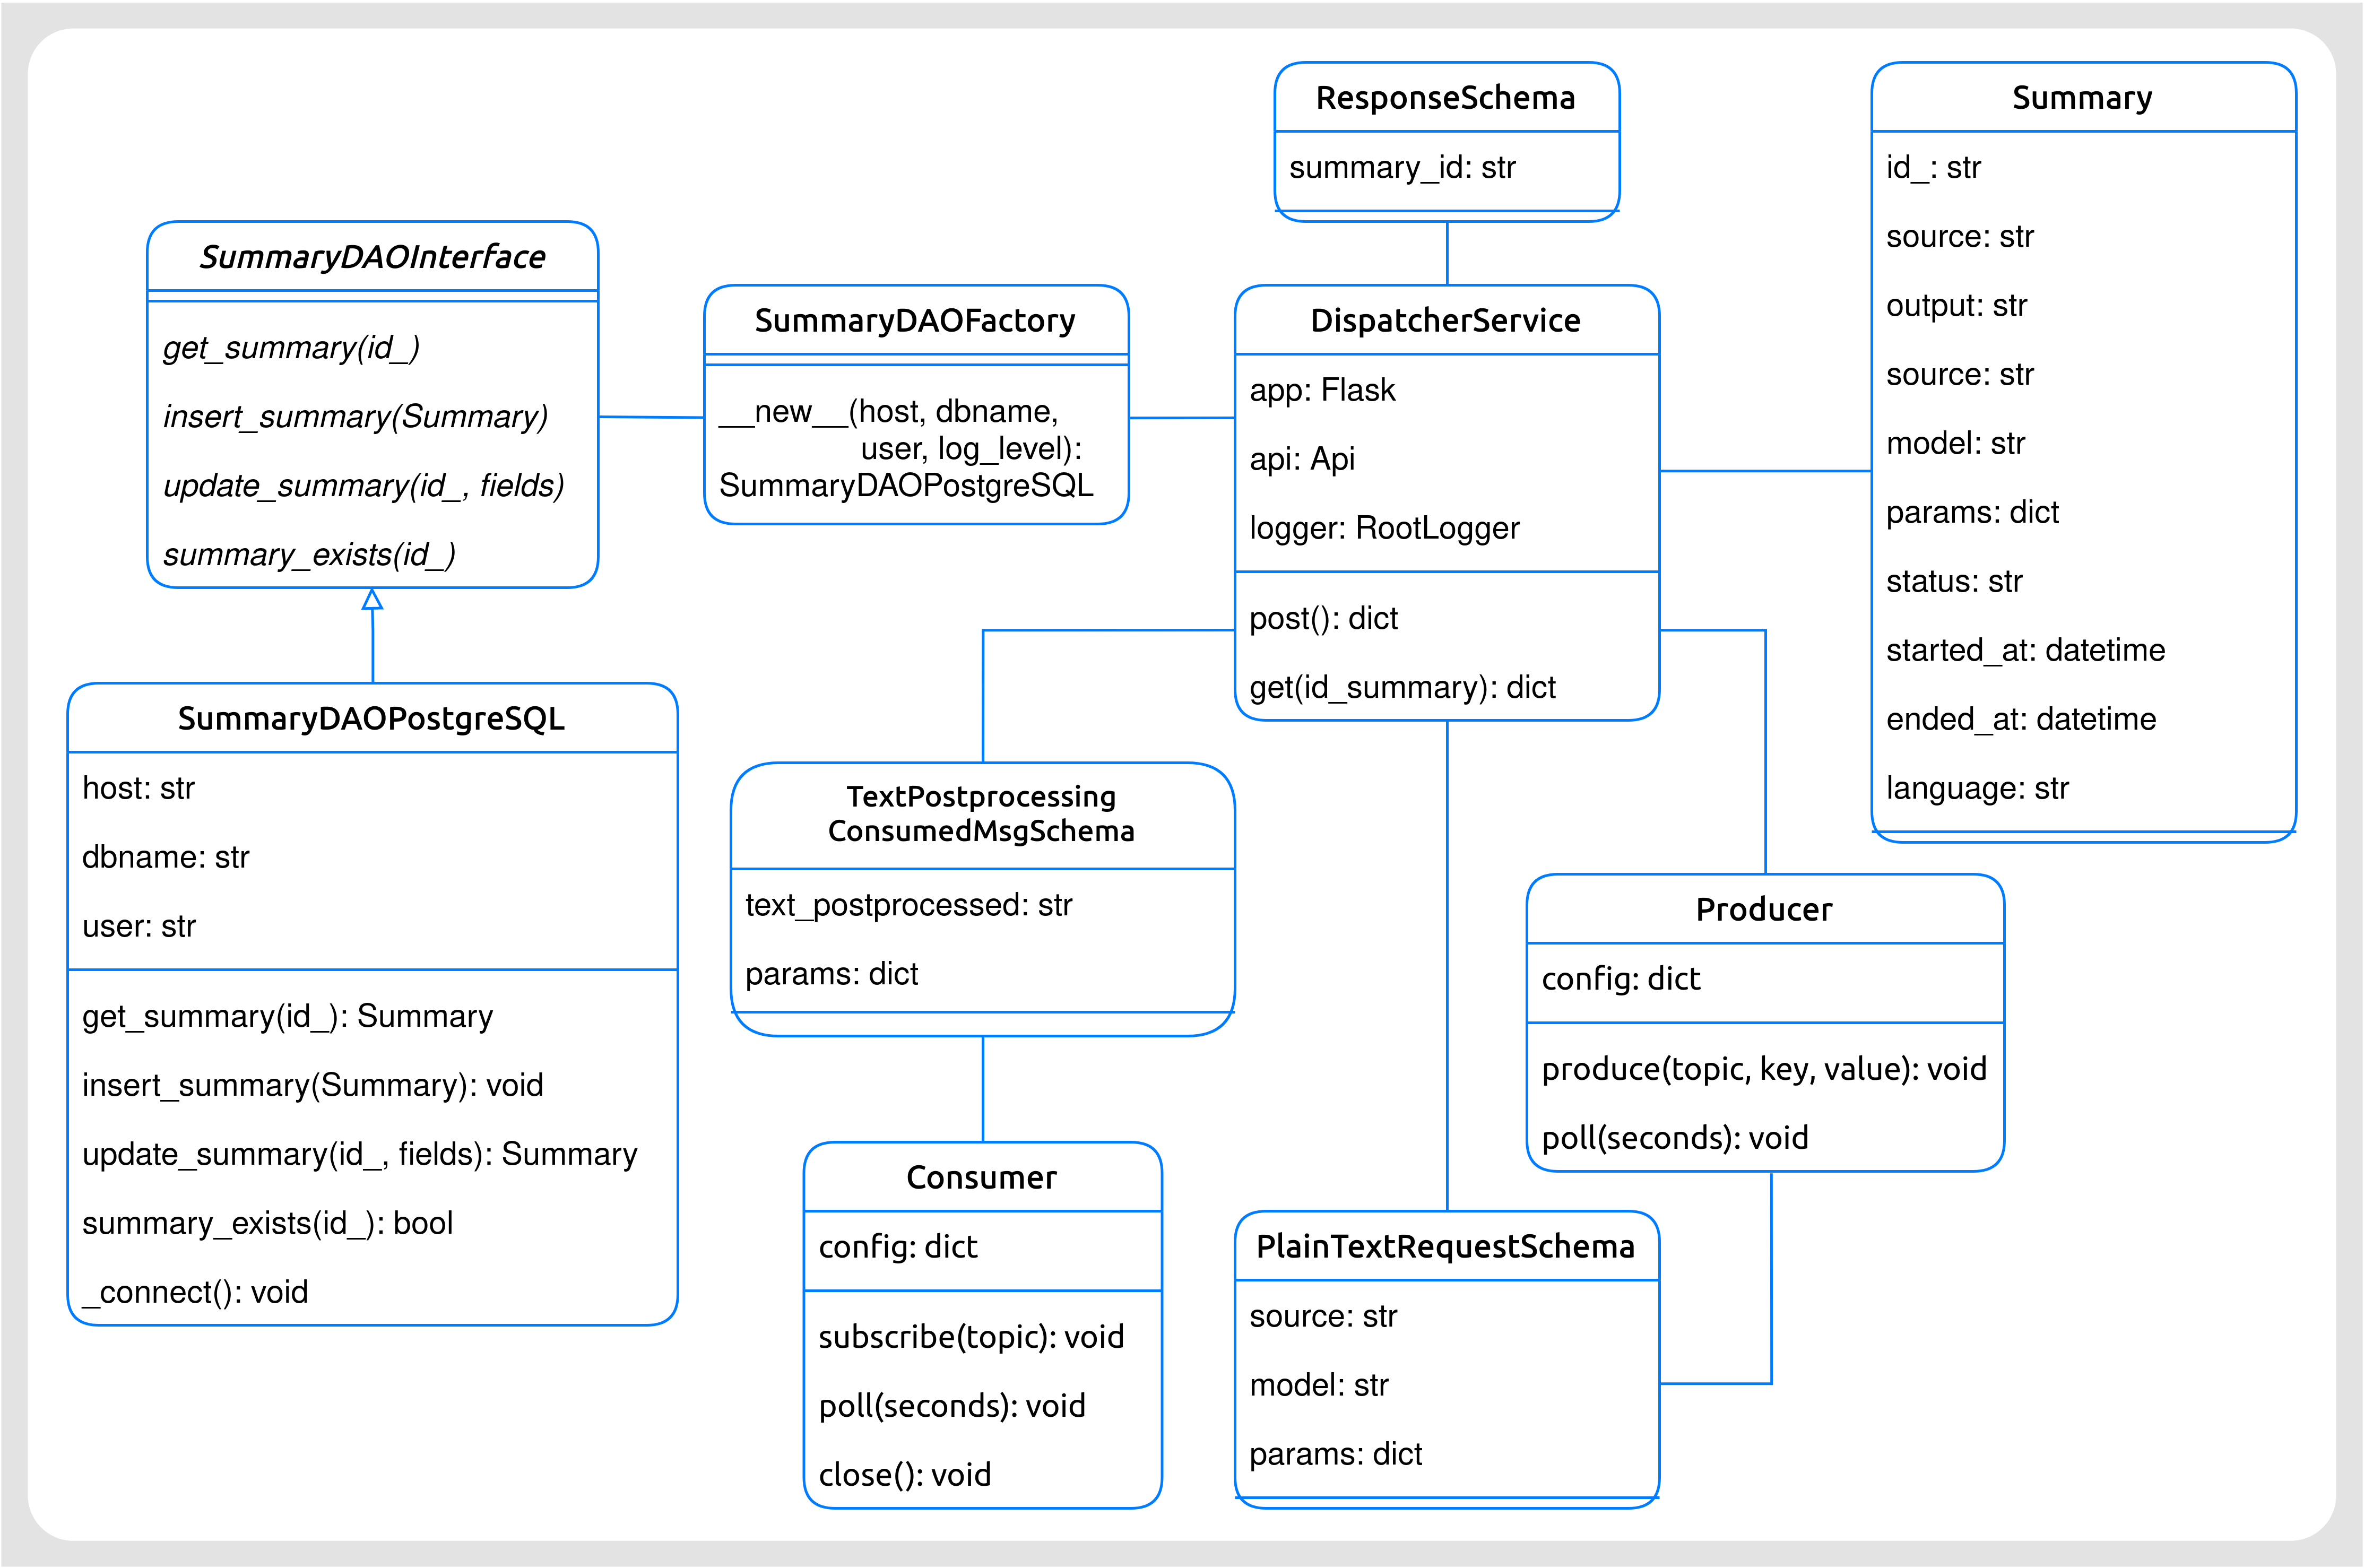
\includegraphics[width=\textwidth]{classes-dispatcher}
	\vspace{-0.5cm}
	\caption{Diagrama de clases del \emph{Dispatcher}.}
\end{figure}

\newpage

\noindent
\textbf{Diagrama E/R de la base de datos}

\begin{figure}[h!]
	\centering
	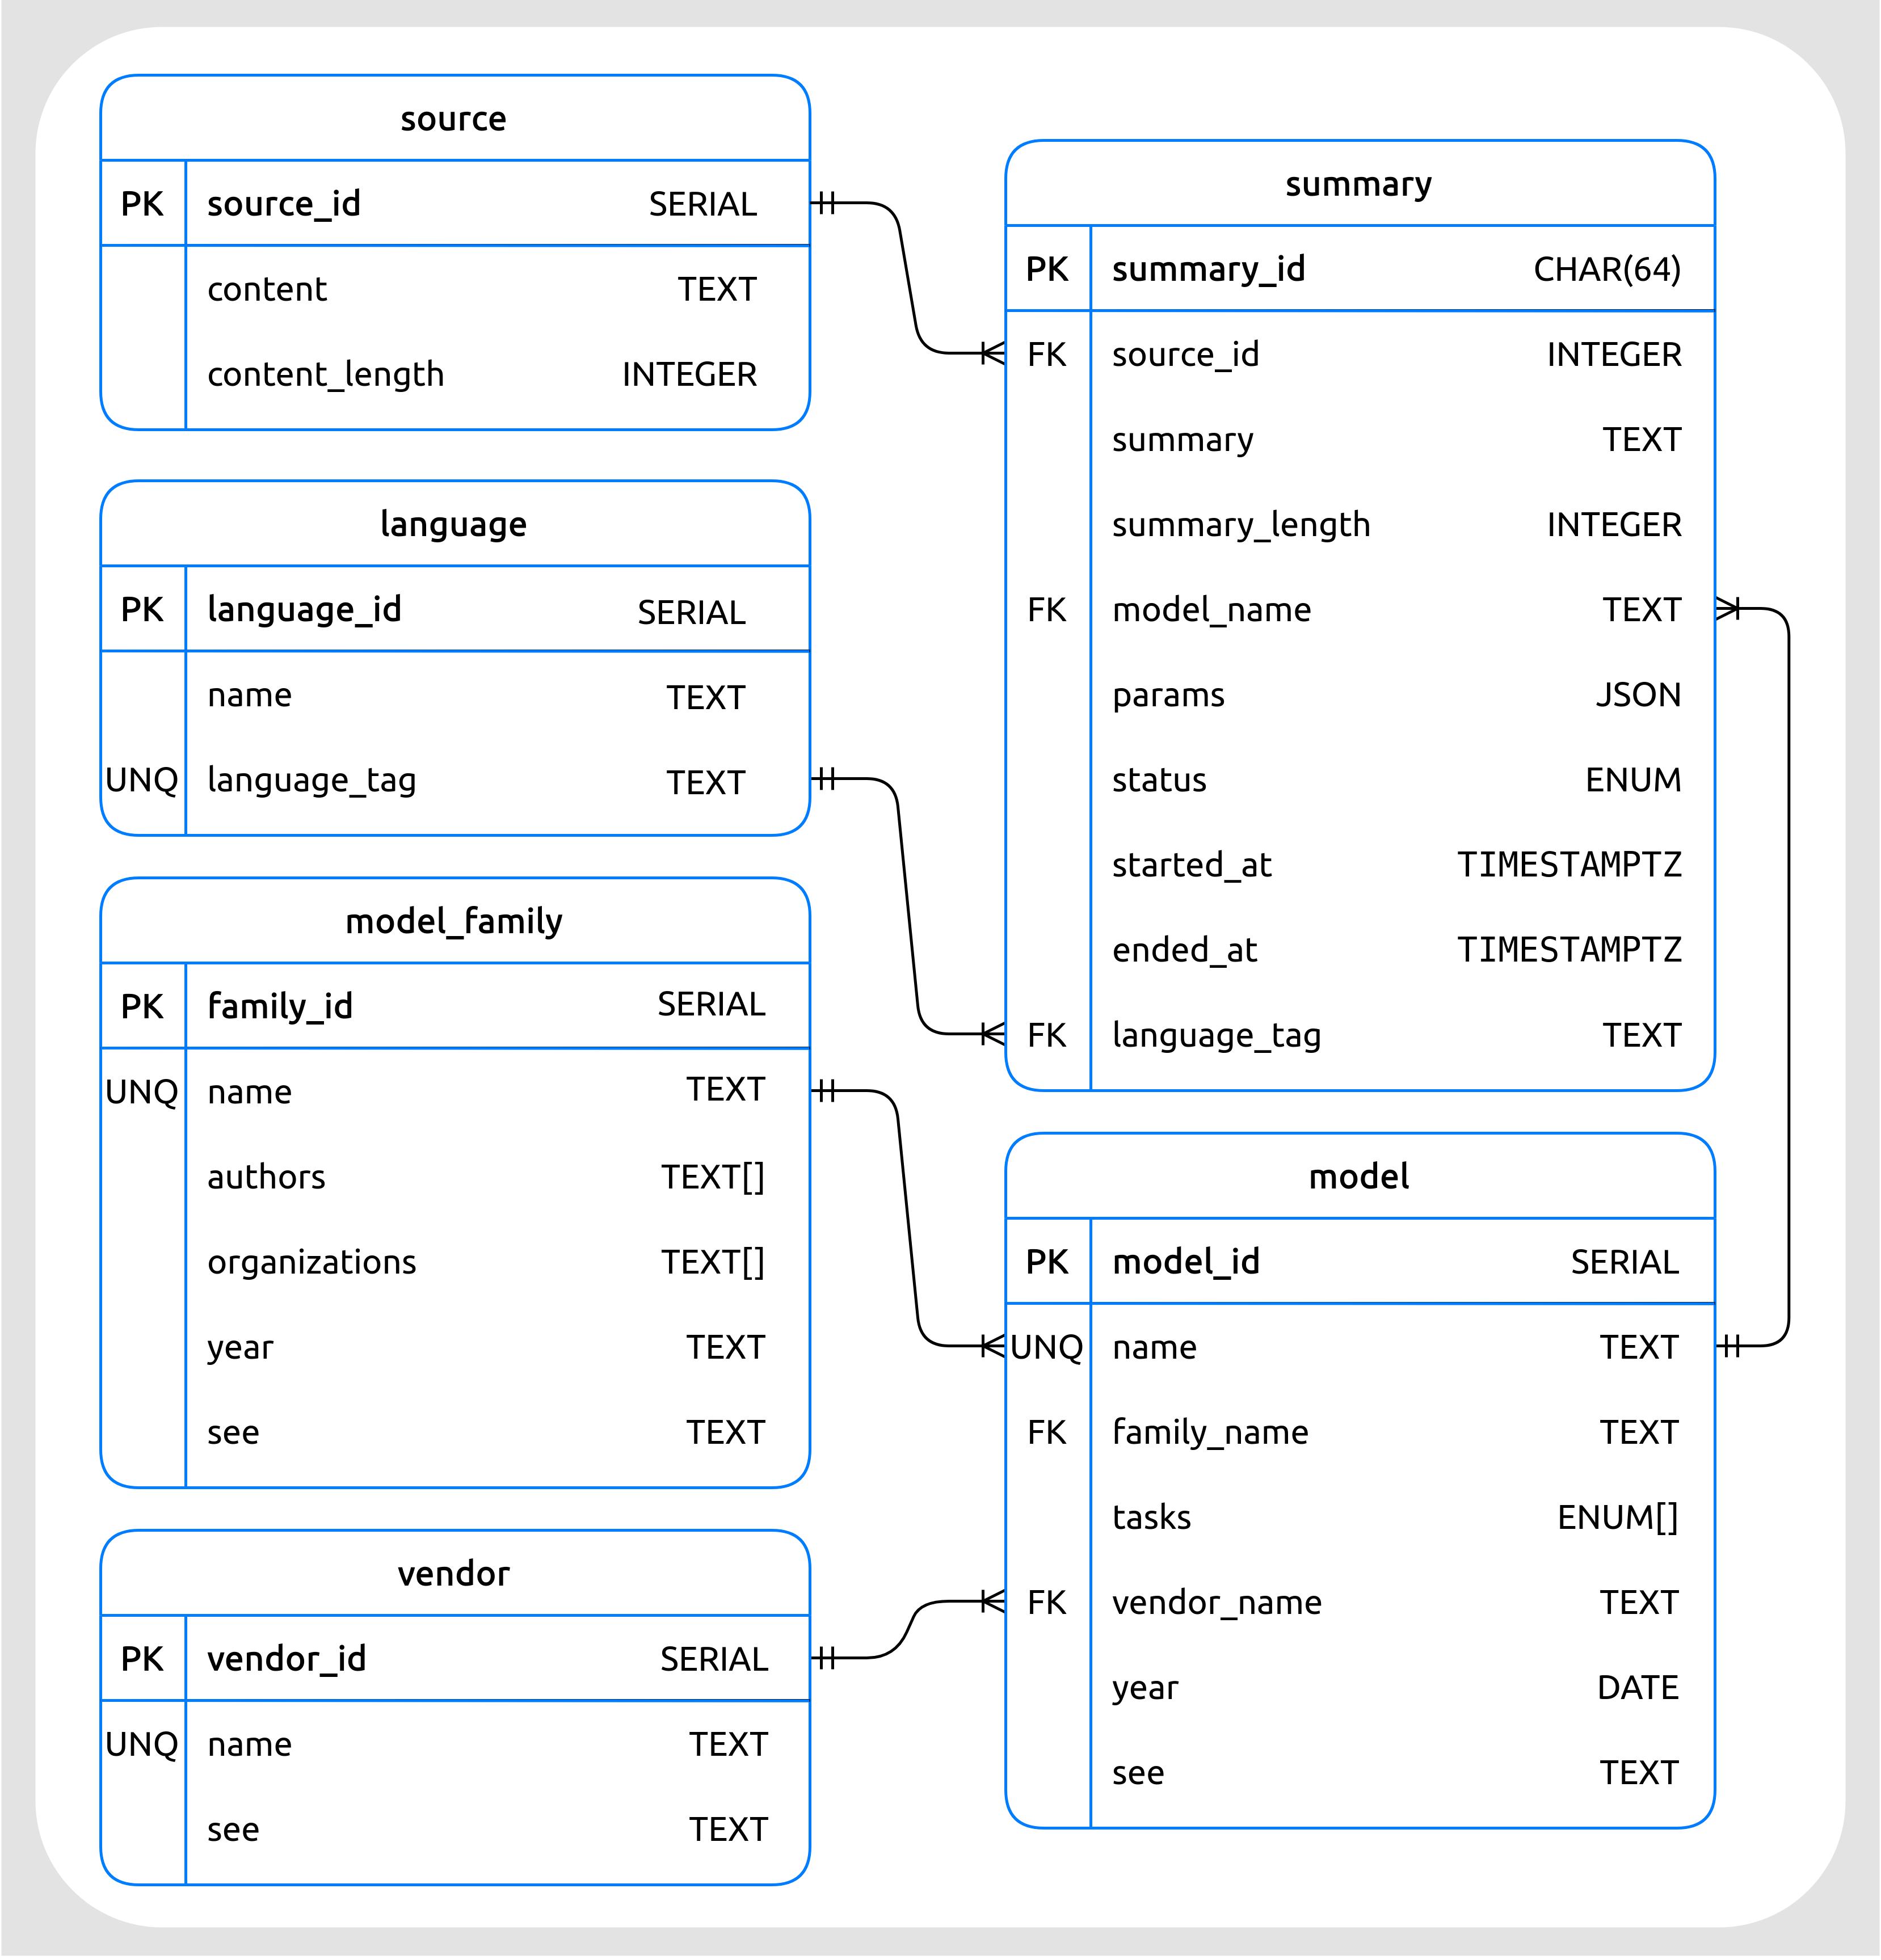
\includegraphics[width=\textwidth]{dispatcher-db}
	\vspace{-0.5cm}
	\caption{Diagrama E/R de la base de datos (tipos de datos de PostgreSQL).}
\end{figure}


\noindent
\textbf{\large Microservicio Pre-procesador de textos}

El Pre-procesador se encarga de realizar un primer procesado de los textos de entrada, a fin de que sean lo más cercanos como sea posible a la entrada que espera el modelo generador de resúmenes.

Este microservicio está compuesto por siguientes clases:

\vspace{-0.2cm}
\begin{itemize} [\textbullet]
	\item \textbf{Pre-procesador de textos (\emph{TextPreprocessor})}: esta clase es la encargada de realizar el pre-procesado del texto.
	
	\item \textbf{Esquema para Mensajes Consumidos \\ (\emph{TextPreprocessingConsumedMsgSchema})}: estructura (campos) que presenta un mensaje consumido por el Pre-procesador. Estos mensajes procederán del microservicio \emph{Dispatcher}.
	
	\item \textbf{Esquema para Mensajes Producidos \\ (\emph{TextEncodingProducedMsgSchema})}: estructura (campos) que presenta un mensaje producido al \emph{topic} del siguiente microservicio (el Codificador de textos).
\end{itemize}

\noindent
\textbf{Diagrama de clases}

\begin{figure}[h]
	\centering
	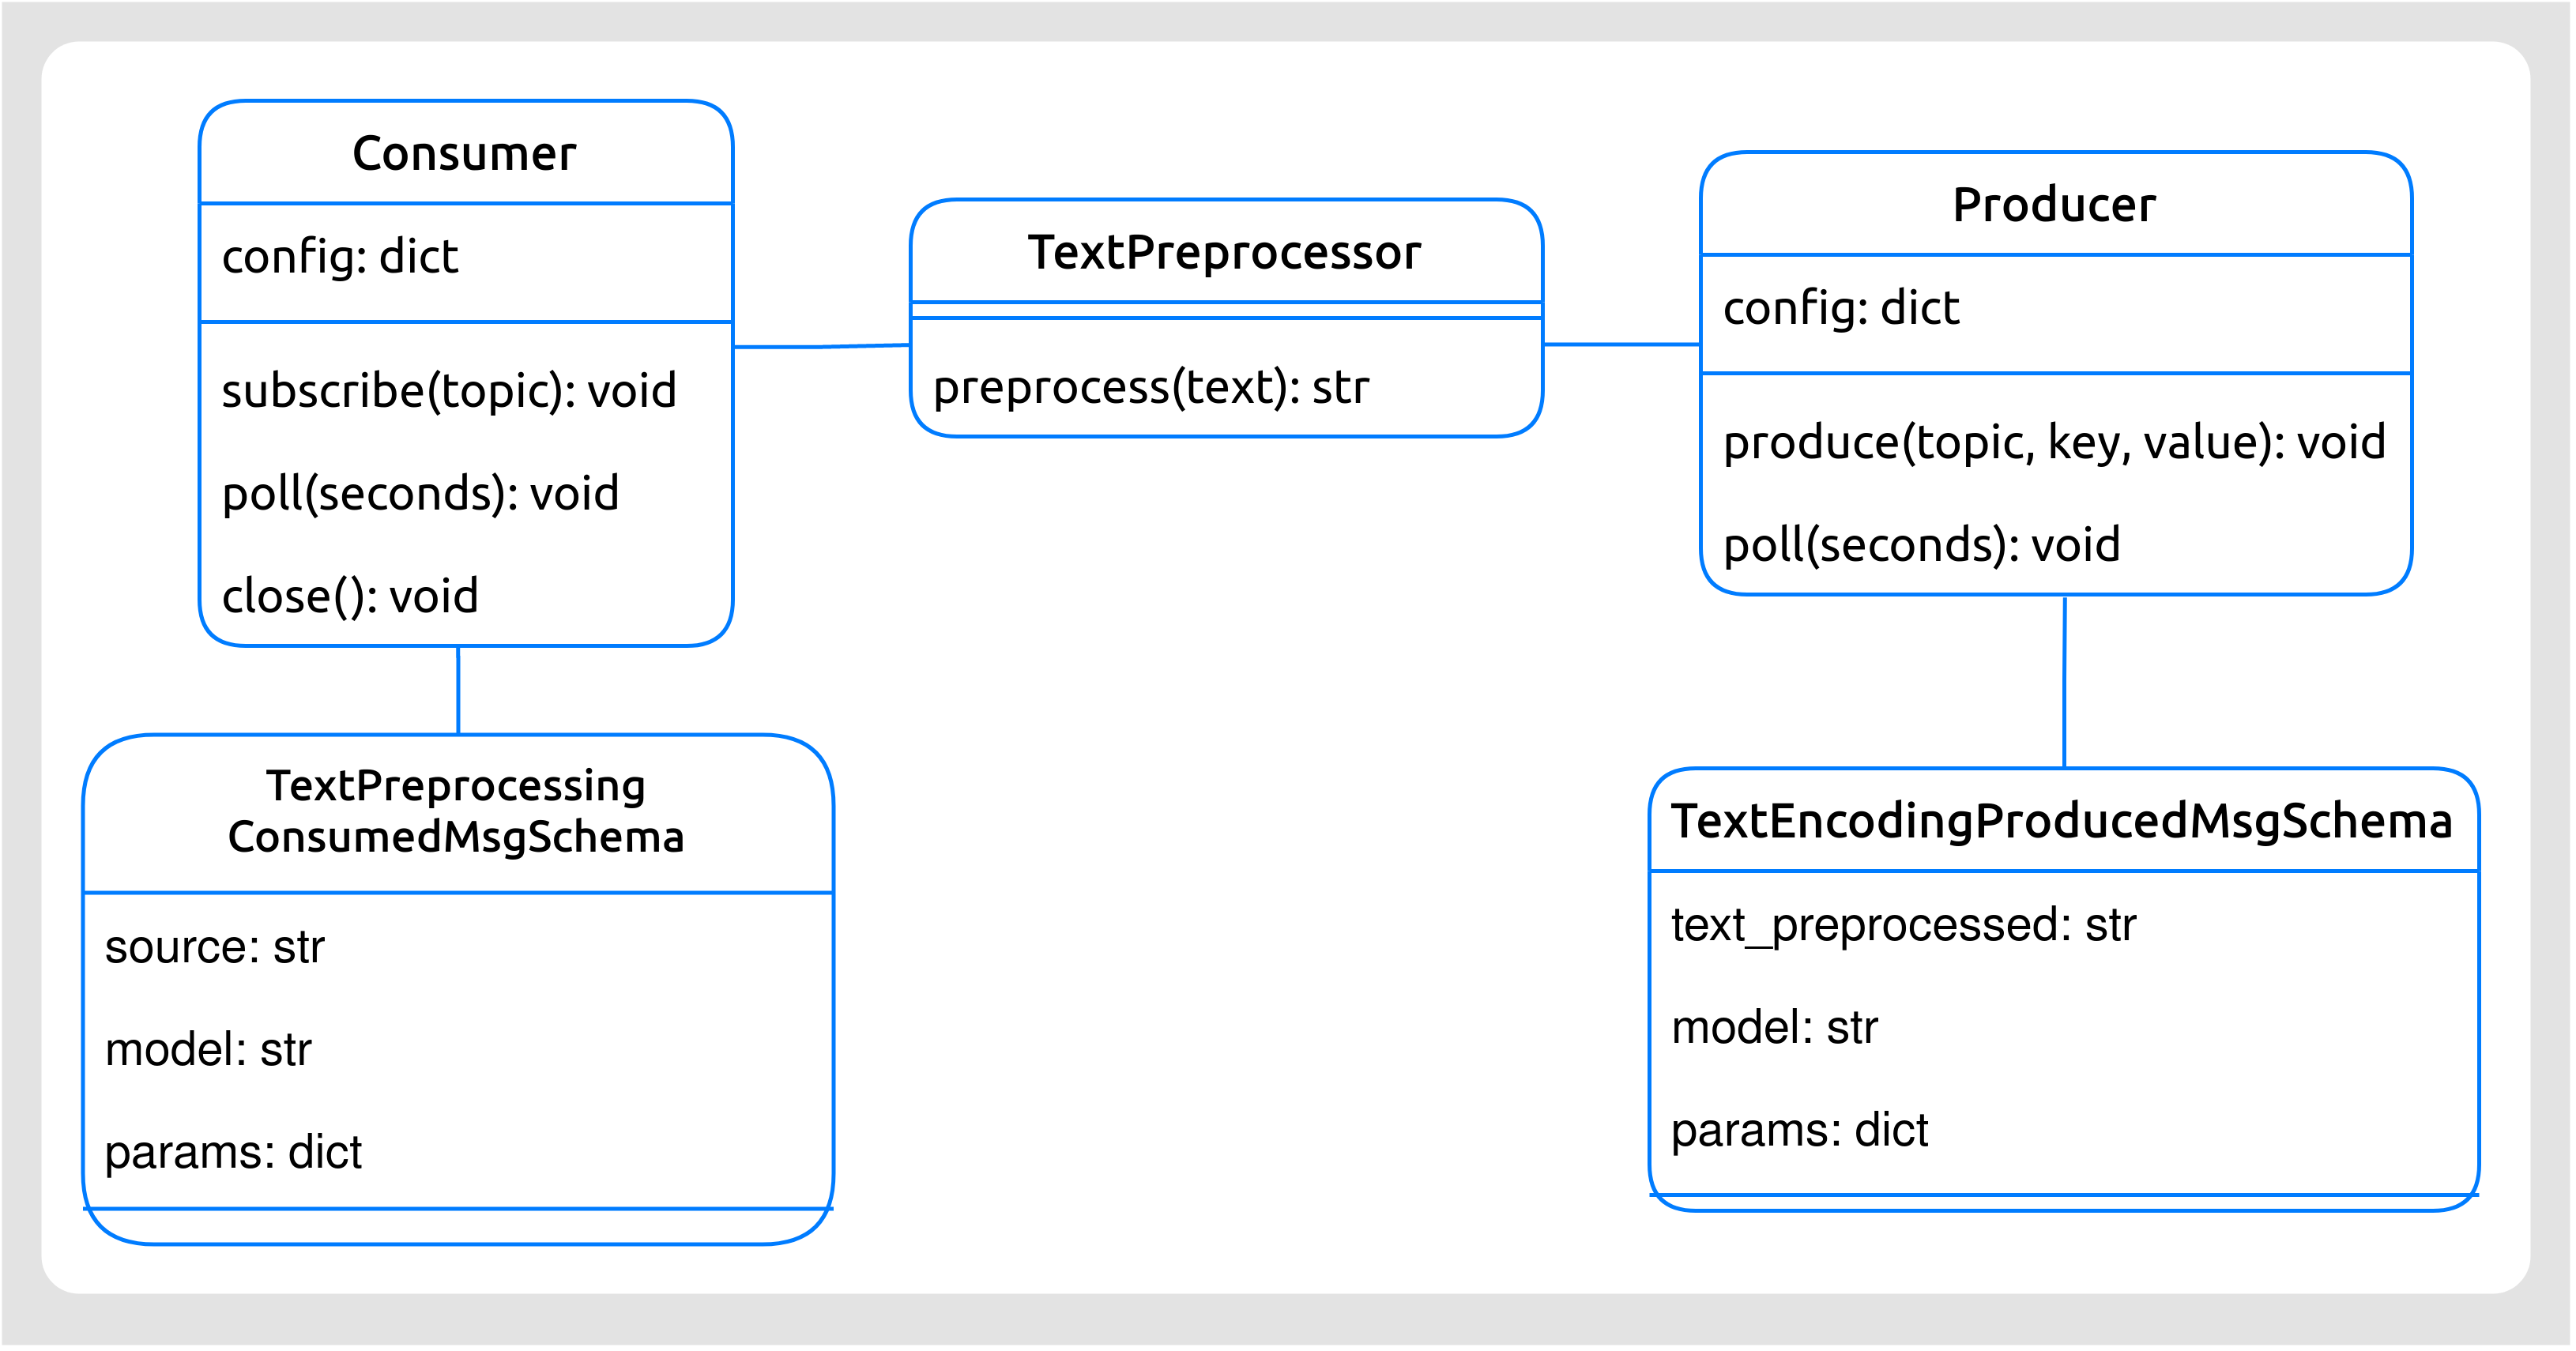
\includegraphics[width=\textwidth]{classes-preprocessor}
	\vspace{-0.5cm}
	\caption{Diagrama de clases del Pre-procesador de textos.}
\end{figure}


\noindent
\textbf{\large Microservicio Codificador de textos}

Este microservicio se encarga de codificar el texto y dividirlo en fragmentos menores, a fin de respetar la longitud máxima de entrada del modelo generador de resúmenes.

El Codificador cuenta con las siguientes clases:

\vspace{-0.2cm}
\begin{itemize} [\textbullet]
	\item \textbf{Codificador y divisor de textos (\emph{SplitterEncoder})}: esta clase es la encargada de realizar el codificado y división del texto.
	
	\item \textbf{Esquema para Mensajes Consumidos \\ (\emph{TextEncodingsConsumedMsgSchema})}: estructura (campos) que presenta un mensaje consumido por el Codificador. Estos mensajes procederán del microservicio Pre-procesador de textos.
	
	\item \textbf{Esquema para Mensajes Producidos \\ (\emph{TextSumarizationProducedMsgSchema})}: estructura (campos) que presenta un mensaje producido al \emph{topic} del siguiente microservicio (el Generador de resumen).
\end{itemize}

\noindent
\textbf{Diagrama de clases}

\begin{figure}[h]
	\centering
	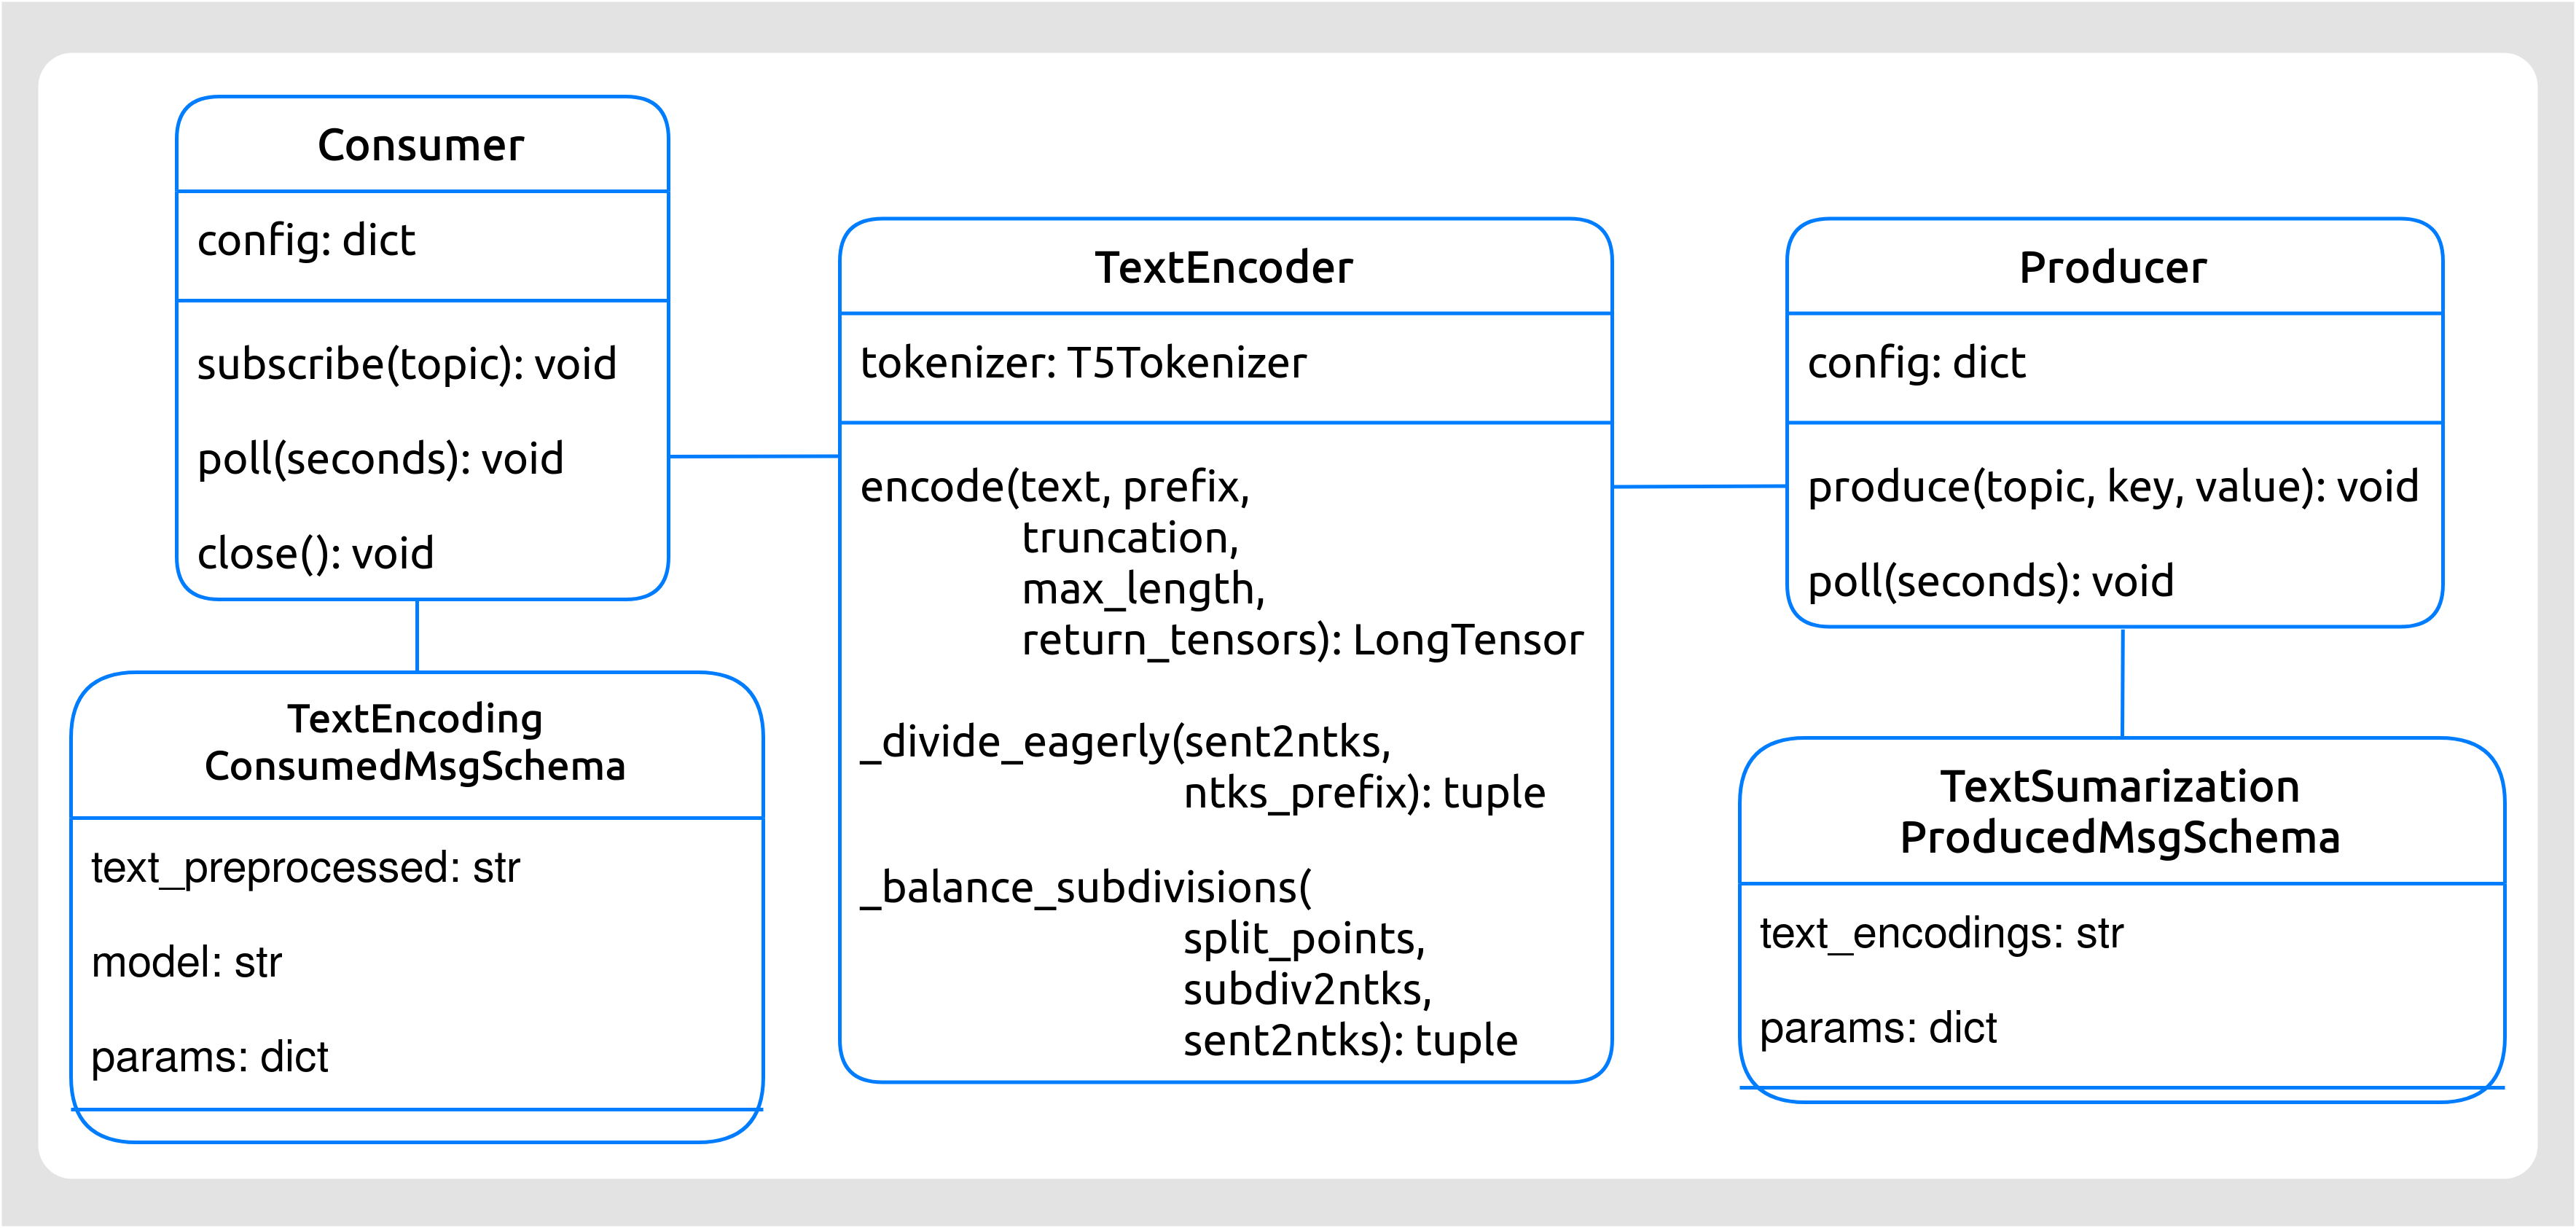
\includegraphics[width=\textwidth]{classes-encoder}
	\vspace{-0.5cm}
	\caption{Diagrama de clases del Codificador de textos.}
\end{figure}


\noindent
\textbf{\large Microservicio Generador de resúmenes}

Este microservicio se encarga de generar resúmenes a partir del texto codificado que recibe del Codificador.

Las clases del Generador de resúmenes son:

\vspace{-0.2cm}
\begin{itemize} [\textbullet]
	\item \textbf{Generador de resúmenes (\emph{Summarizer})}: esta clase es la encargada de generar los resúmenes.
	
	\item \textbf{Esquema para Mensajes Consumidos \\ (\emph{TextSummarizationConsumedMsgSchema})}: estructura (campos) que presenta un mensaje consumido por el Generador de resúmenes. Estos mensajes procederán del microservicio Codificador de textos.
	
	\item \textbf{Esquema para Mensajes Producidos \\ (\emph{TextPostprocessingProducedMsgSchema})}: estructura (campos) que presenta un mensaje producido al \emph{topic} del siguiente microservicio (el Post-procesador de textos).
\end{itemize}

\noindent
\textbf{Diagrama de clases}

\begin{figure}[h]
	\centering
	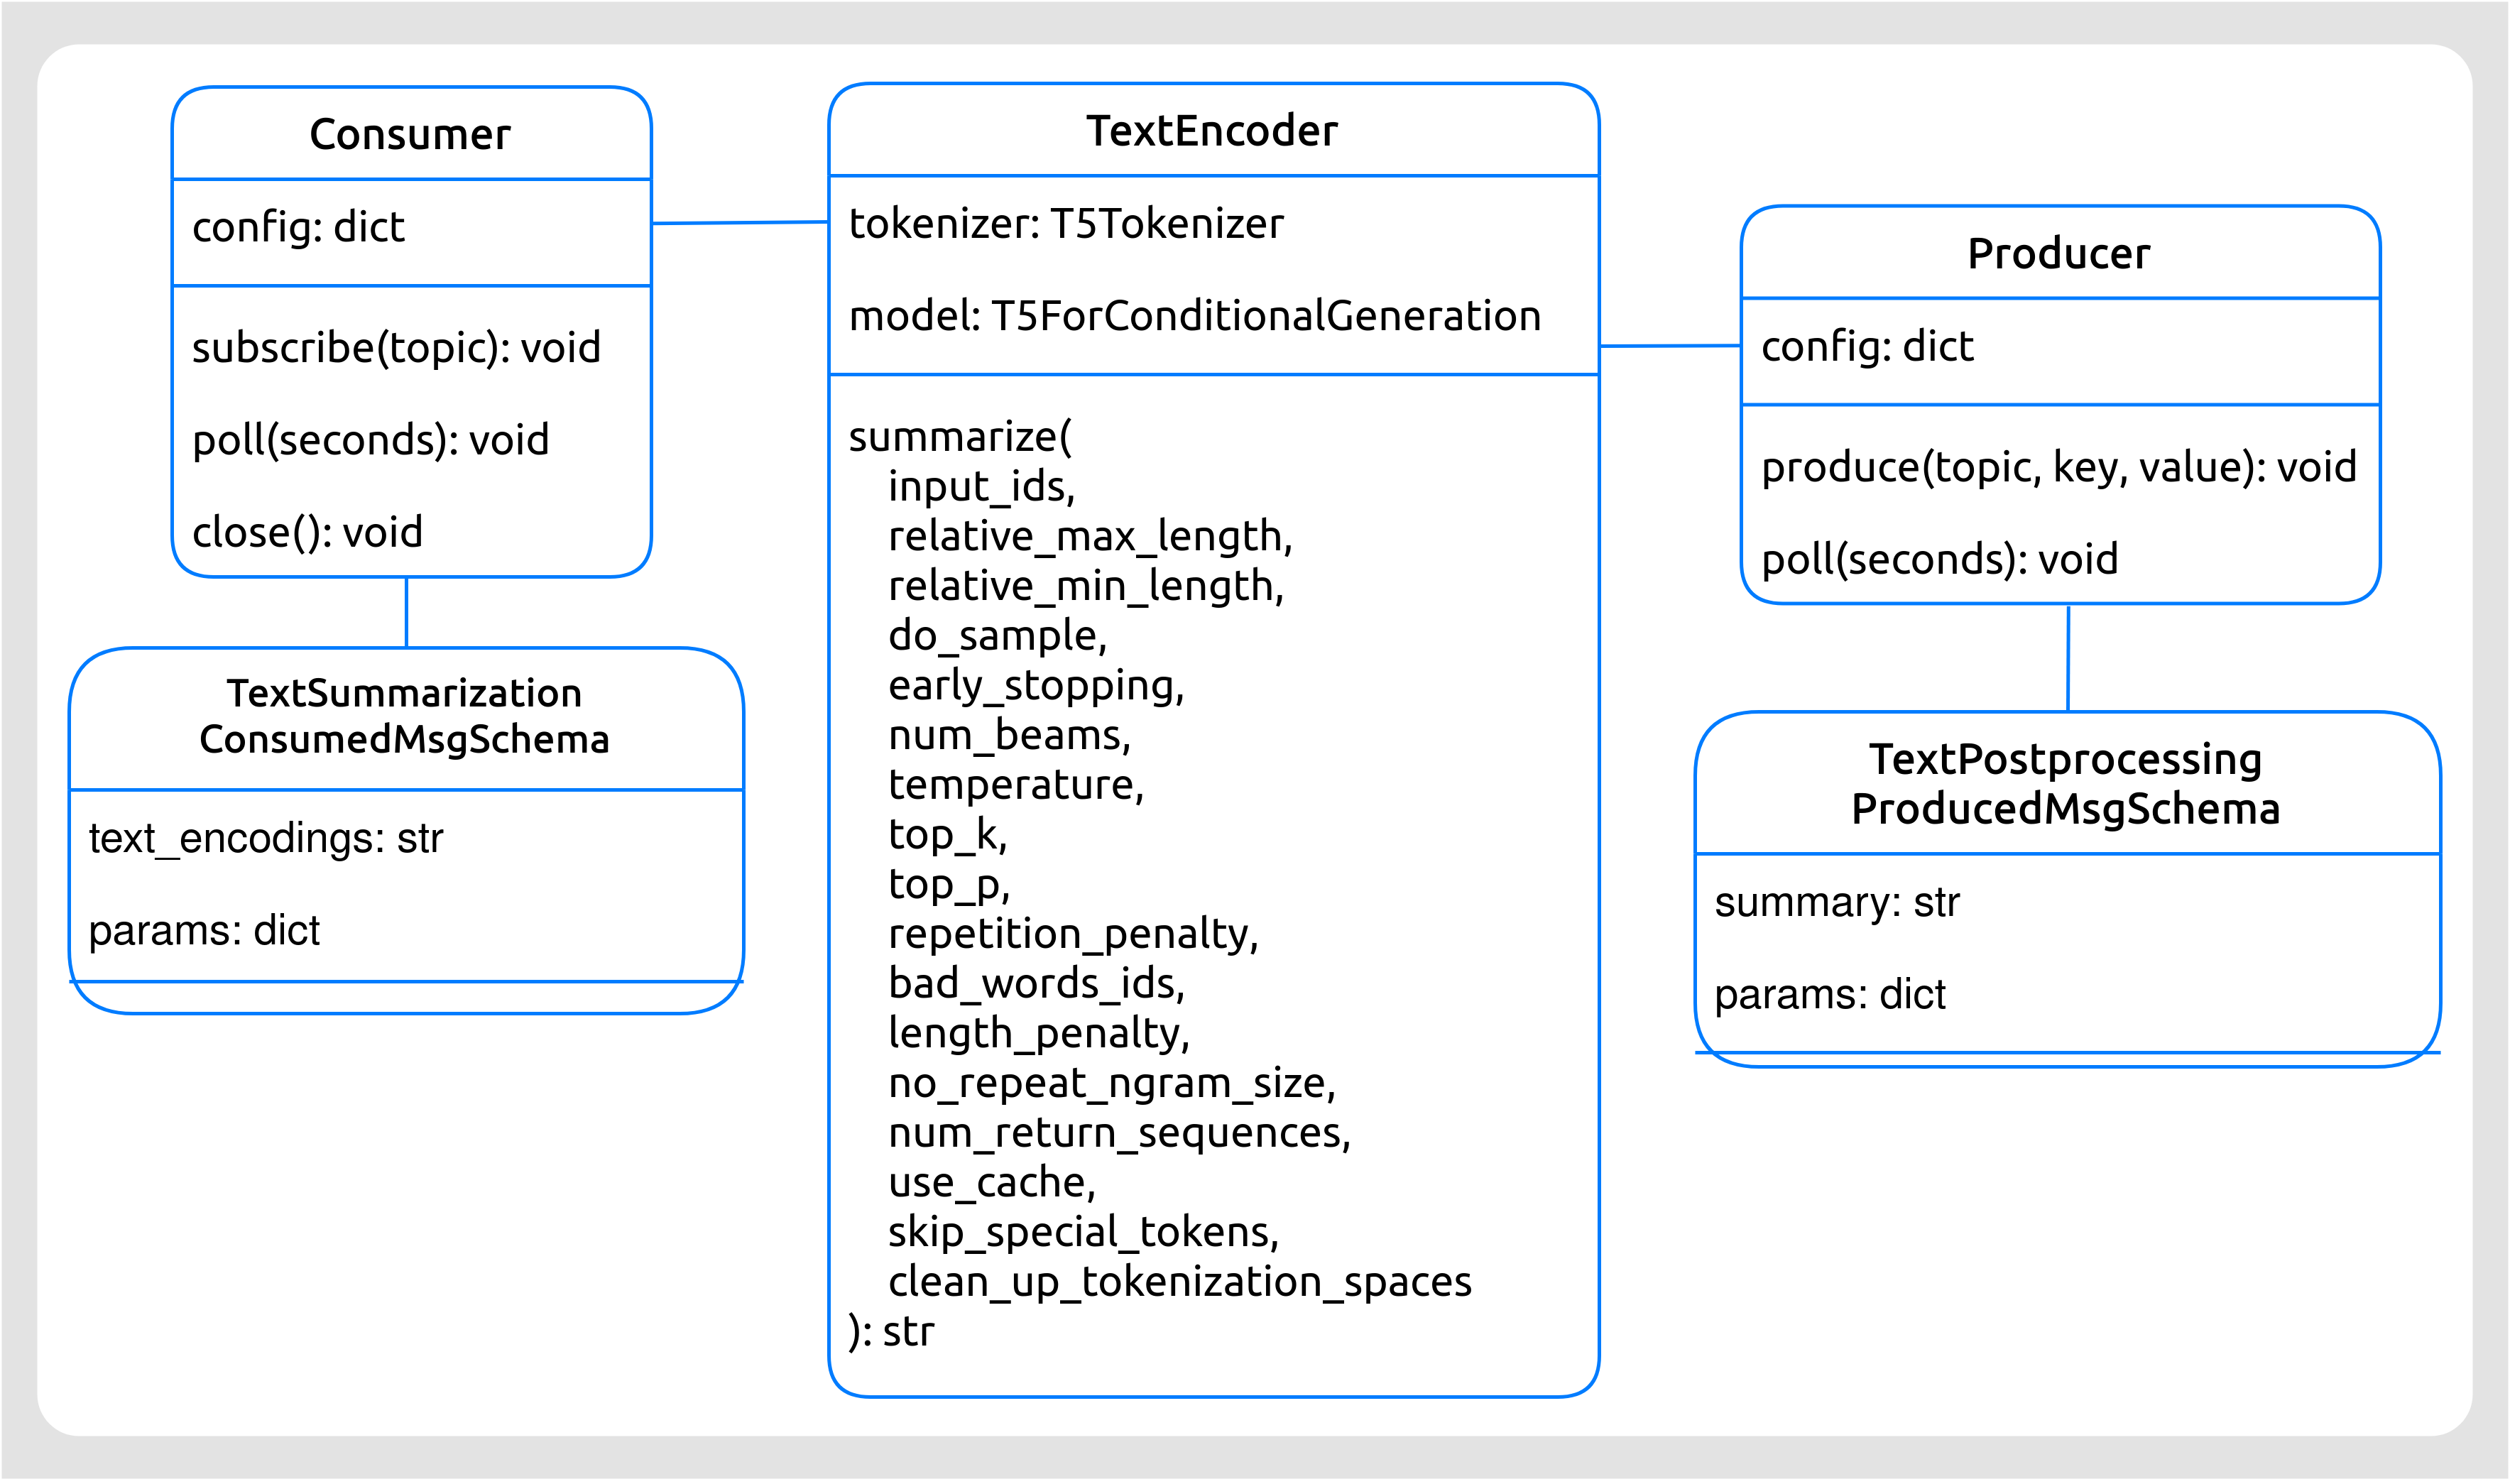
\includegraphics[width=\textwidth]{classes-summarizer}
	\vspace{-0.5cm}
	\caption{Diagrama de clases del Generador de resúmenes.}
\end{figure}



\noindent
\textbf{\large Microservicio Post-procesador de textos}

Este microservicio lleva a cabo el post-procesado del resumen entregado por el Generador de resúmenes.

El Post-procesador de textos tiene las siguientes clases.

\vspace{-0.2cm}
\begin{itemize} [\textbullet]
	\item \textbf{Post-procesador de textos (\emph{TextPostprocessor})}: esta clase es la encargada de post-procesar el texto.
	
	\item \textbf{Esquema para Mensajes Consumidos \\ (\emph{TextPostprocessingConsumedMsgSchema})}: estructura (campos) que presenta un mensaje consumido por el Post-procesador de textos. Estos mensajes procederán del microservicio Generador de resúmenes.
	
	\item \textbf{Esquema para Mensajes Producidos \\ (\emph{ReadyProducedMsgSchema})}: estructura (campos) que presenta un mensaje producido al siguiente \emph{topic}, \emph{Ready}.
\end{itemize}

\noindent
\textbf{Diagrama de clases}

\begin{figure}[h]
	\centering
	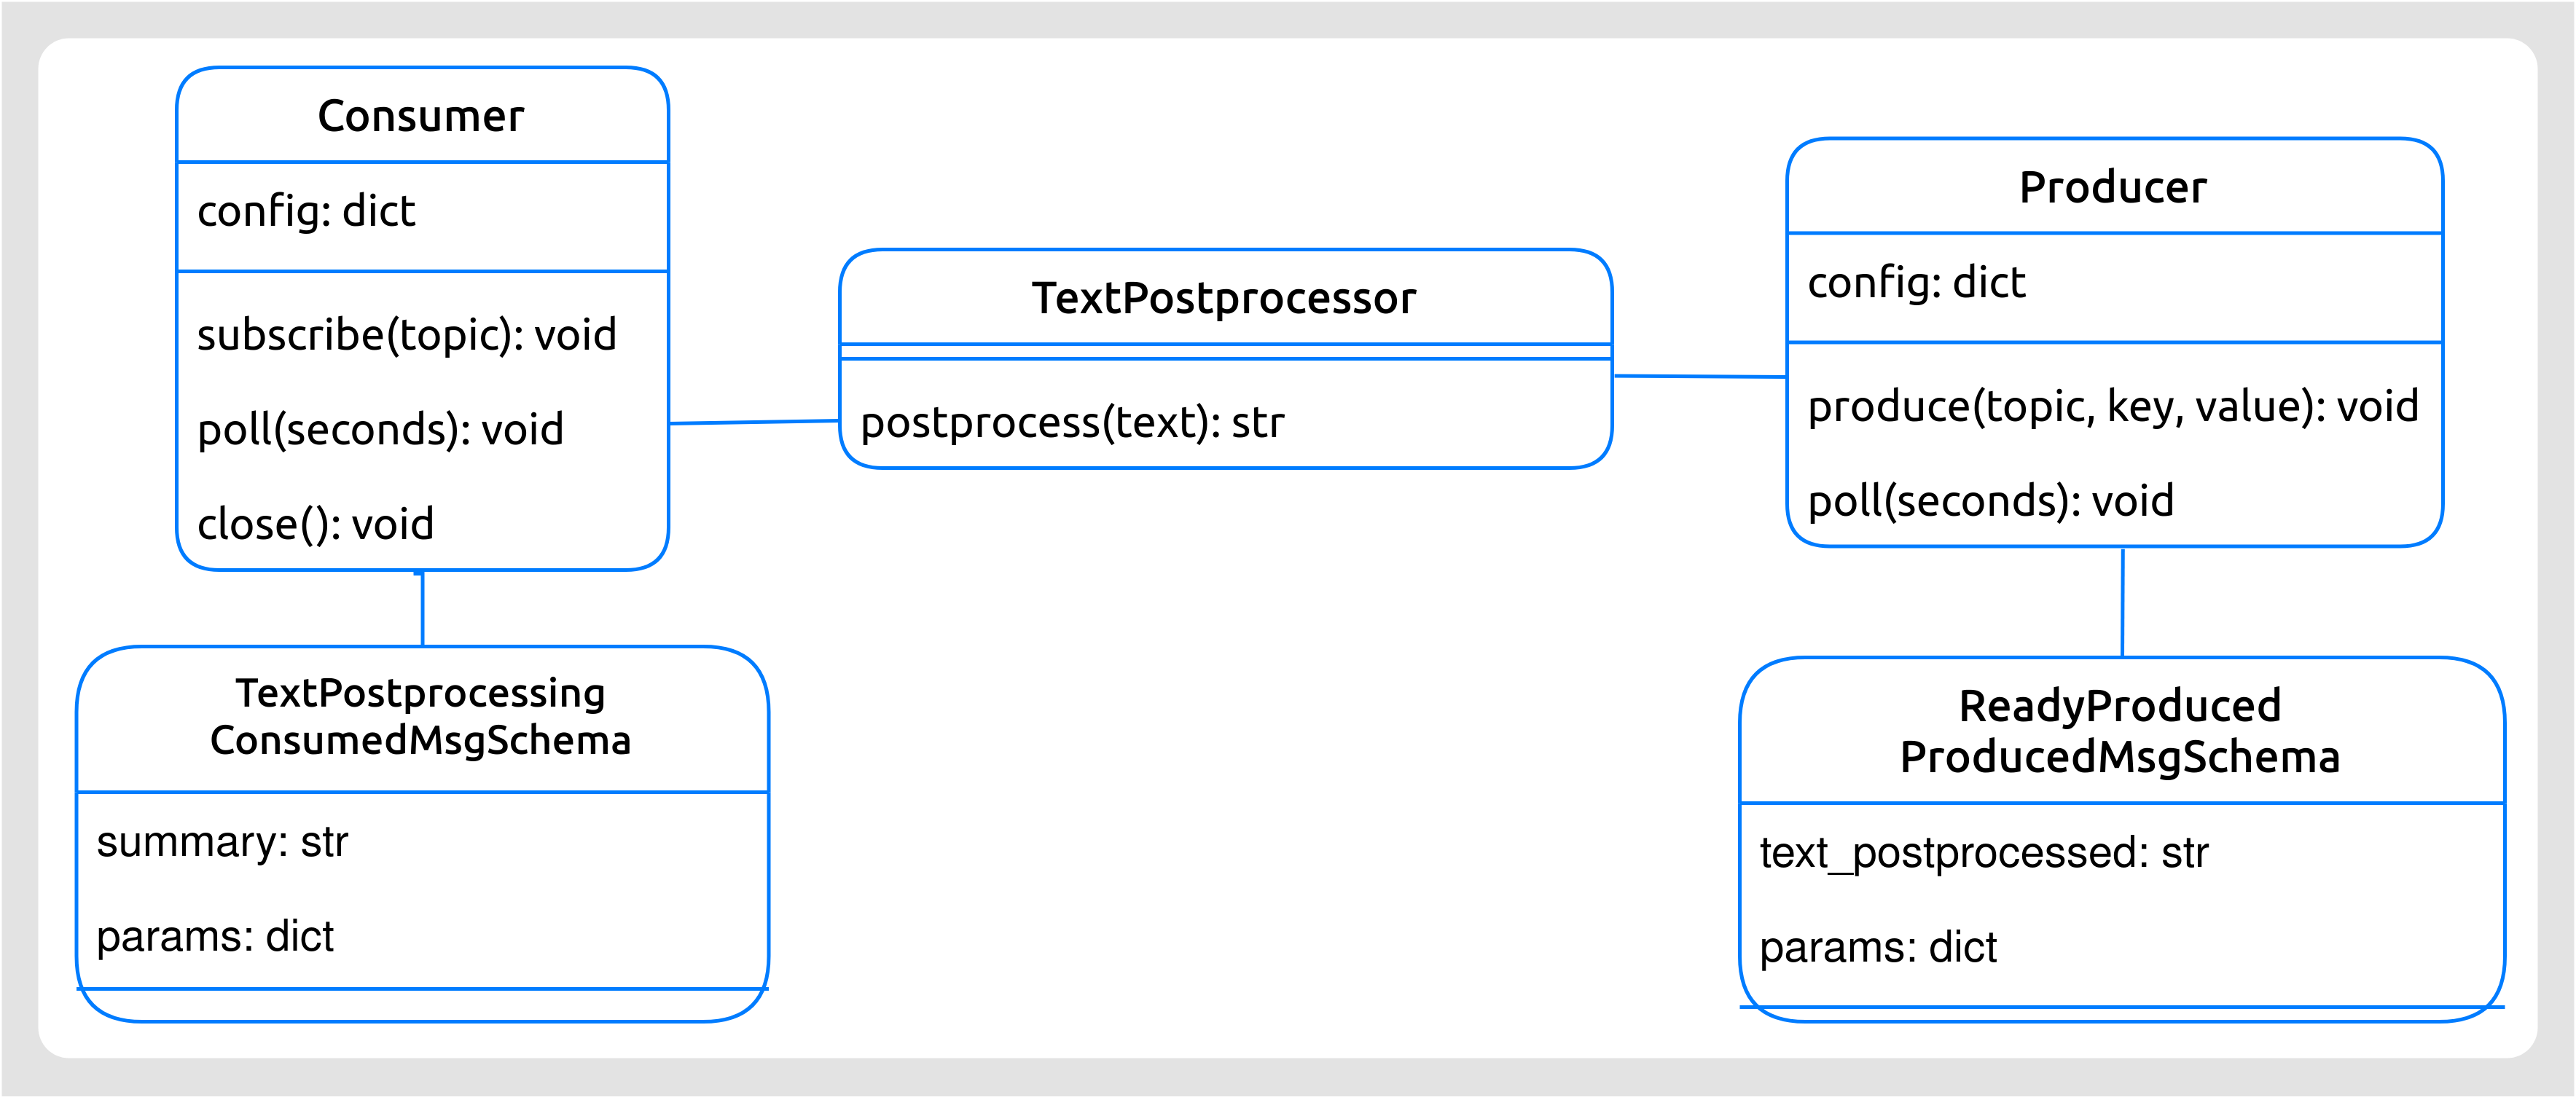
\includegraphics[width=\textwidth]{classes-postprocessor}
	\vspace{-0.5cm}
	\caption{Diagrama de clases del Post-procesador de textos.}
\end{figure}


\subsubsection{\Large \emph{Frontend}}

El \emph{frontend} está compuesto por la aplicación multiplataforma desarrollada siguiendo los patrones de \emph{Clean Architectura} y Diseño guiado por el dominio \emph{Domain Driven Design}. Para conocer los detalles concretos de la implementación de la arquitectura de la \emph{app}, se recomienda acudir a la sección ``Motivación tras las arquitecturas desarrolladas'' del capítulo ``Aspectos relevantes'' de la Memoria.

Las clases identificadas en la aplicación son las siguientes:

\vspace{-0.2cm}
\begin{itemize} [\textbullet]
	\item \textbf{JiztApp}: esta clase representa la aplicación en su conjunto. En el \texttt{main} de la aplicación, se ejecuta una instancia de esta clase.
	
	\item \textbf{NewSummaryPage}: se corresponde con la pantalla desde la cual los usuarios pueden solicitar nuevos resúmenes.
	
	\item \textbf{SummaryPage}: se corresponde con la pantalla en la que se muestra el resumen generado.
	
	\item \textbf{NewSummaryCubit}: clase encargada de transformar los eventos procedentes de los usuarios en la pantalla \texttt{NewSummaryPage} (por ejemplo, un \emph{click}), en acciones particulares de la aplicación.
	
	\item \textbf{SummaryCubit}: análoga a la anterior solo que en este caso para la pantalla \texttt{SummaryPage}.
	
	\item \textbf{JiztRepository}: clase que encapsula y centraliza la lógica de acceso a las fuentes de datos.
	
	\item \textbf{JiztCacheClient}: clase que gestiona el acceso a la base de datos local.
	
	\item \textbf{JiztApiClient}: clase que gestiona la comunicación con la REST API de JIZT.
	
	\item \textbf{Summary}: representa un resumen. En realidad, disponemos de tres representaciones de un resumen, cada una correspondiéndose con cada uno de los dominios (capa de dominio, caché y REST API). No obstante, la estructura de las mismas es análoga; por consiguiente, las sintetizamos todas en una única clase para simplificar el esquema de diseño.
\end{itemize}


\begin{figure}[h]
	\centering
	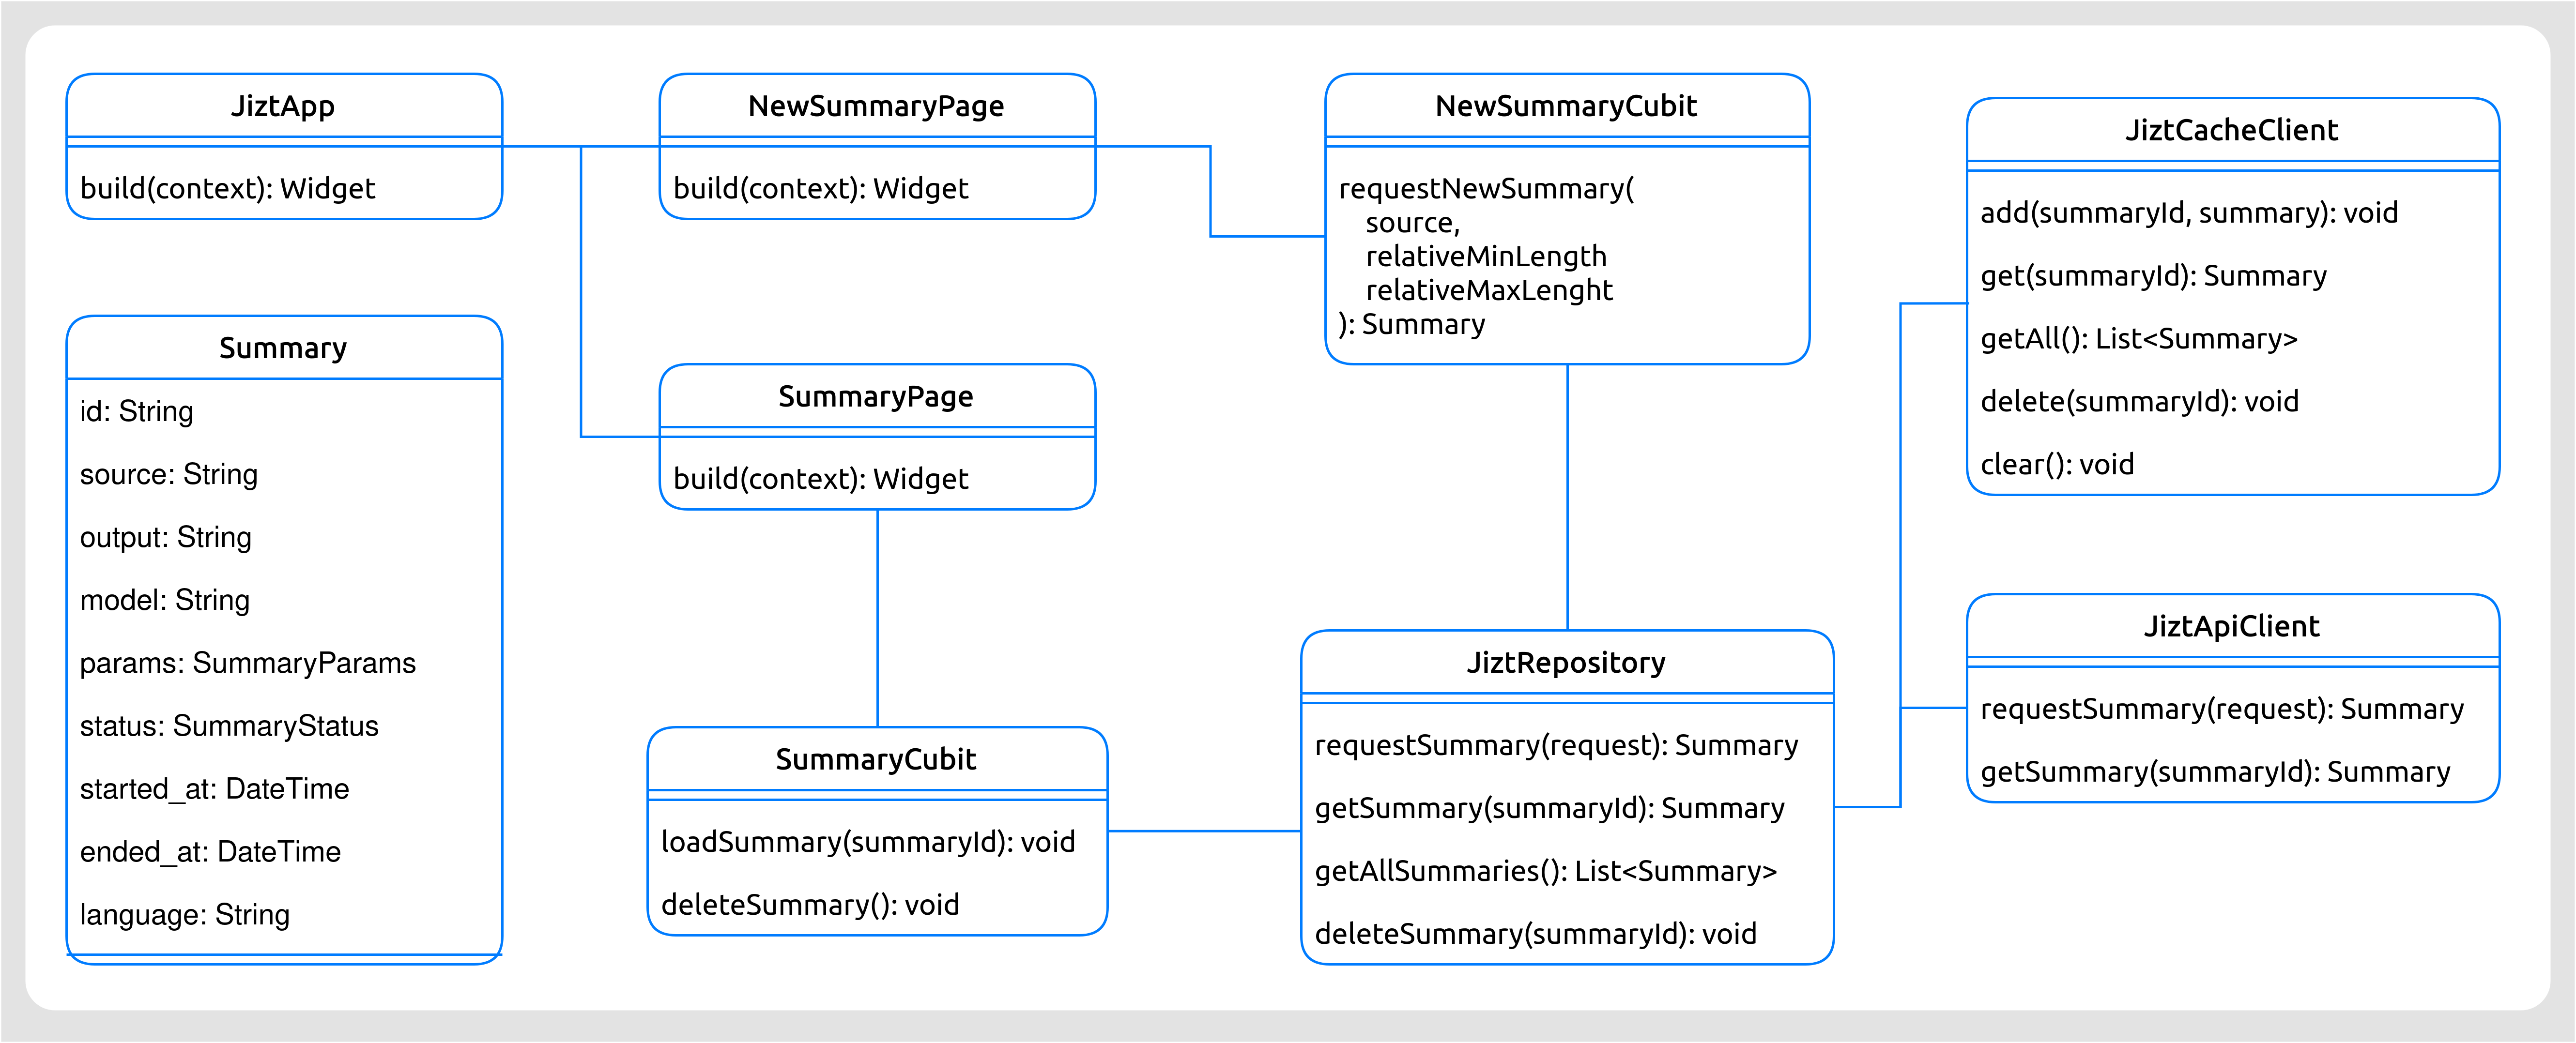
\includegraphics[width=\textwidth]{classes-app}
	\vspace{-0.5cm}
	\caption{Diagrama de clases de la aplicación de JIZT.}
\end{figure}


\section{Diseño procedimental}

En esta sección repasamos una vez más los pasos que se llevan a cabo tanto en el \emph{backend} a la hora de atender las peticiones de los clientes y generar los resúmenes, como en la aplicación, encargada de gestionar los resúmenes de los usuarios.

En la sección correspondiente al \emph{backend} del capítulo ``Técnicas y Herramientas'', explicábamos cómo se gestionaba la comunicación entre los clientes y la REST API a través de peticiones HTTP. Recordemos el proceso:

\begin{enumerate}
	\item El cliente realiza una petición HTTP POST, incluyendo en el cuerpo el texto a resumir, así como los parámetros del resumen a generar.
	
	\item Ingress (API \emph{Gateway}) comprueba que dicha petición se está haciendo a un \emph{endpoint} válido, y en ese caso la redirige hacia el \emph{Dispatcher}.
	
	\item El \emph{Dispatcher} realiza una serie de comprobaciones:
	\begin{enumerate}	
		\item Se consulta en la base de datos si ya existe un resumen generado para ese texto con esos parámetros. En ese caso, se responde al cliente con los datos del resumen (\texttt{output}, \texttt{source}, \texttt{started\_at}, \texttt{ended\_at}, etc.).
		
		\item En caso contrario, se responde con el mismo esquema de datos, solo que el \texttt{output} será \texttt{null}. Al mismo tiempo, se produce un mensaje al \emph{topic} del pre-procesador de textos, conteniendo el texto y los parámetros del resumen, comenzando el proceso de generación.
	\end{enumerate}
	
	\item El pre-procesador está constantemente comprobando si existen mensajes nuevos en su \emph{topic}. En ese caso los consume, realiza las tareas de pre-procesado, y produce el resultado en el \emph{topic} del codificador.
	
	\item Este proceso continua de forma análoga hasta llegar al post-procesador, el cual produce el resumen final al \emph{topic} <<Listo>> (\emph{Ready}). El \emph{Dispatcher}, en ese momento, consume el mensaje, y actualiza la base de datos.
	
	\item Mientras el proceso de resumen se completa, el cliente realiza peticiones GET de manera periódica, hasta que la API REST finalmente responde con el resumen generado.
\end{enumerate}

La \autoref{seq-app} ilustra este proceso de forma gráfica, a través de un diagrama de secuencia.

A su vez, en la aplicación, es decir, el \emph{frontend}, de llevan a cabo los siguientes pasos:

\begin{enumerate}
	\item El usuario solicita generar un nuevo resumen, pulsando para ello sobre la pantalla.
	
	\item El evento se transforma a través del \emph{cubit} en un petición de resumen al repositorio.
	
	\item El repositorio realiza una petición HTTP POST al \emph{backend} para obtener el \emph{id} del resumen a partir del texto fuente, los parámetros del resumen, y el modelo.
	
	\item Una vez obtenido el \emph{id} del resumen, se consulta la base de datos local (capa de caché) para conocer si ya se dispone localmente del resumen solicitado. En ese caso, se devuelve el resumen, y se actualiza la pantalla para mostrárselo al usuario.
	
	\item En caso contario, se realiza peticiones GET periódicas a la API REST hasta que el resumen se completa. Finalmente, se actualiza la pantalla.
\end{enumerate}

En la \autoref{seq-app}, se incluye un diagrama de clases que describe el proceso de manera más detallada.

\vspace{1cm}

\begin{figure}[h]
	\centering
	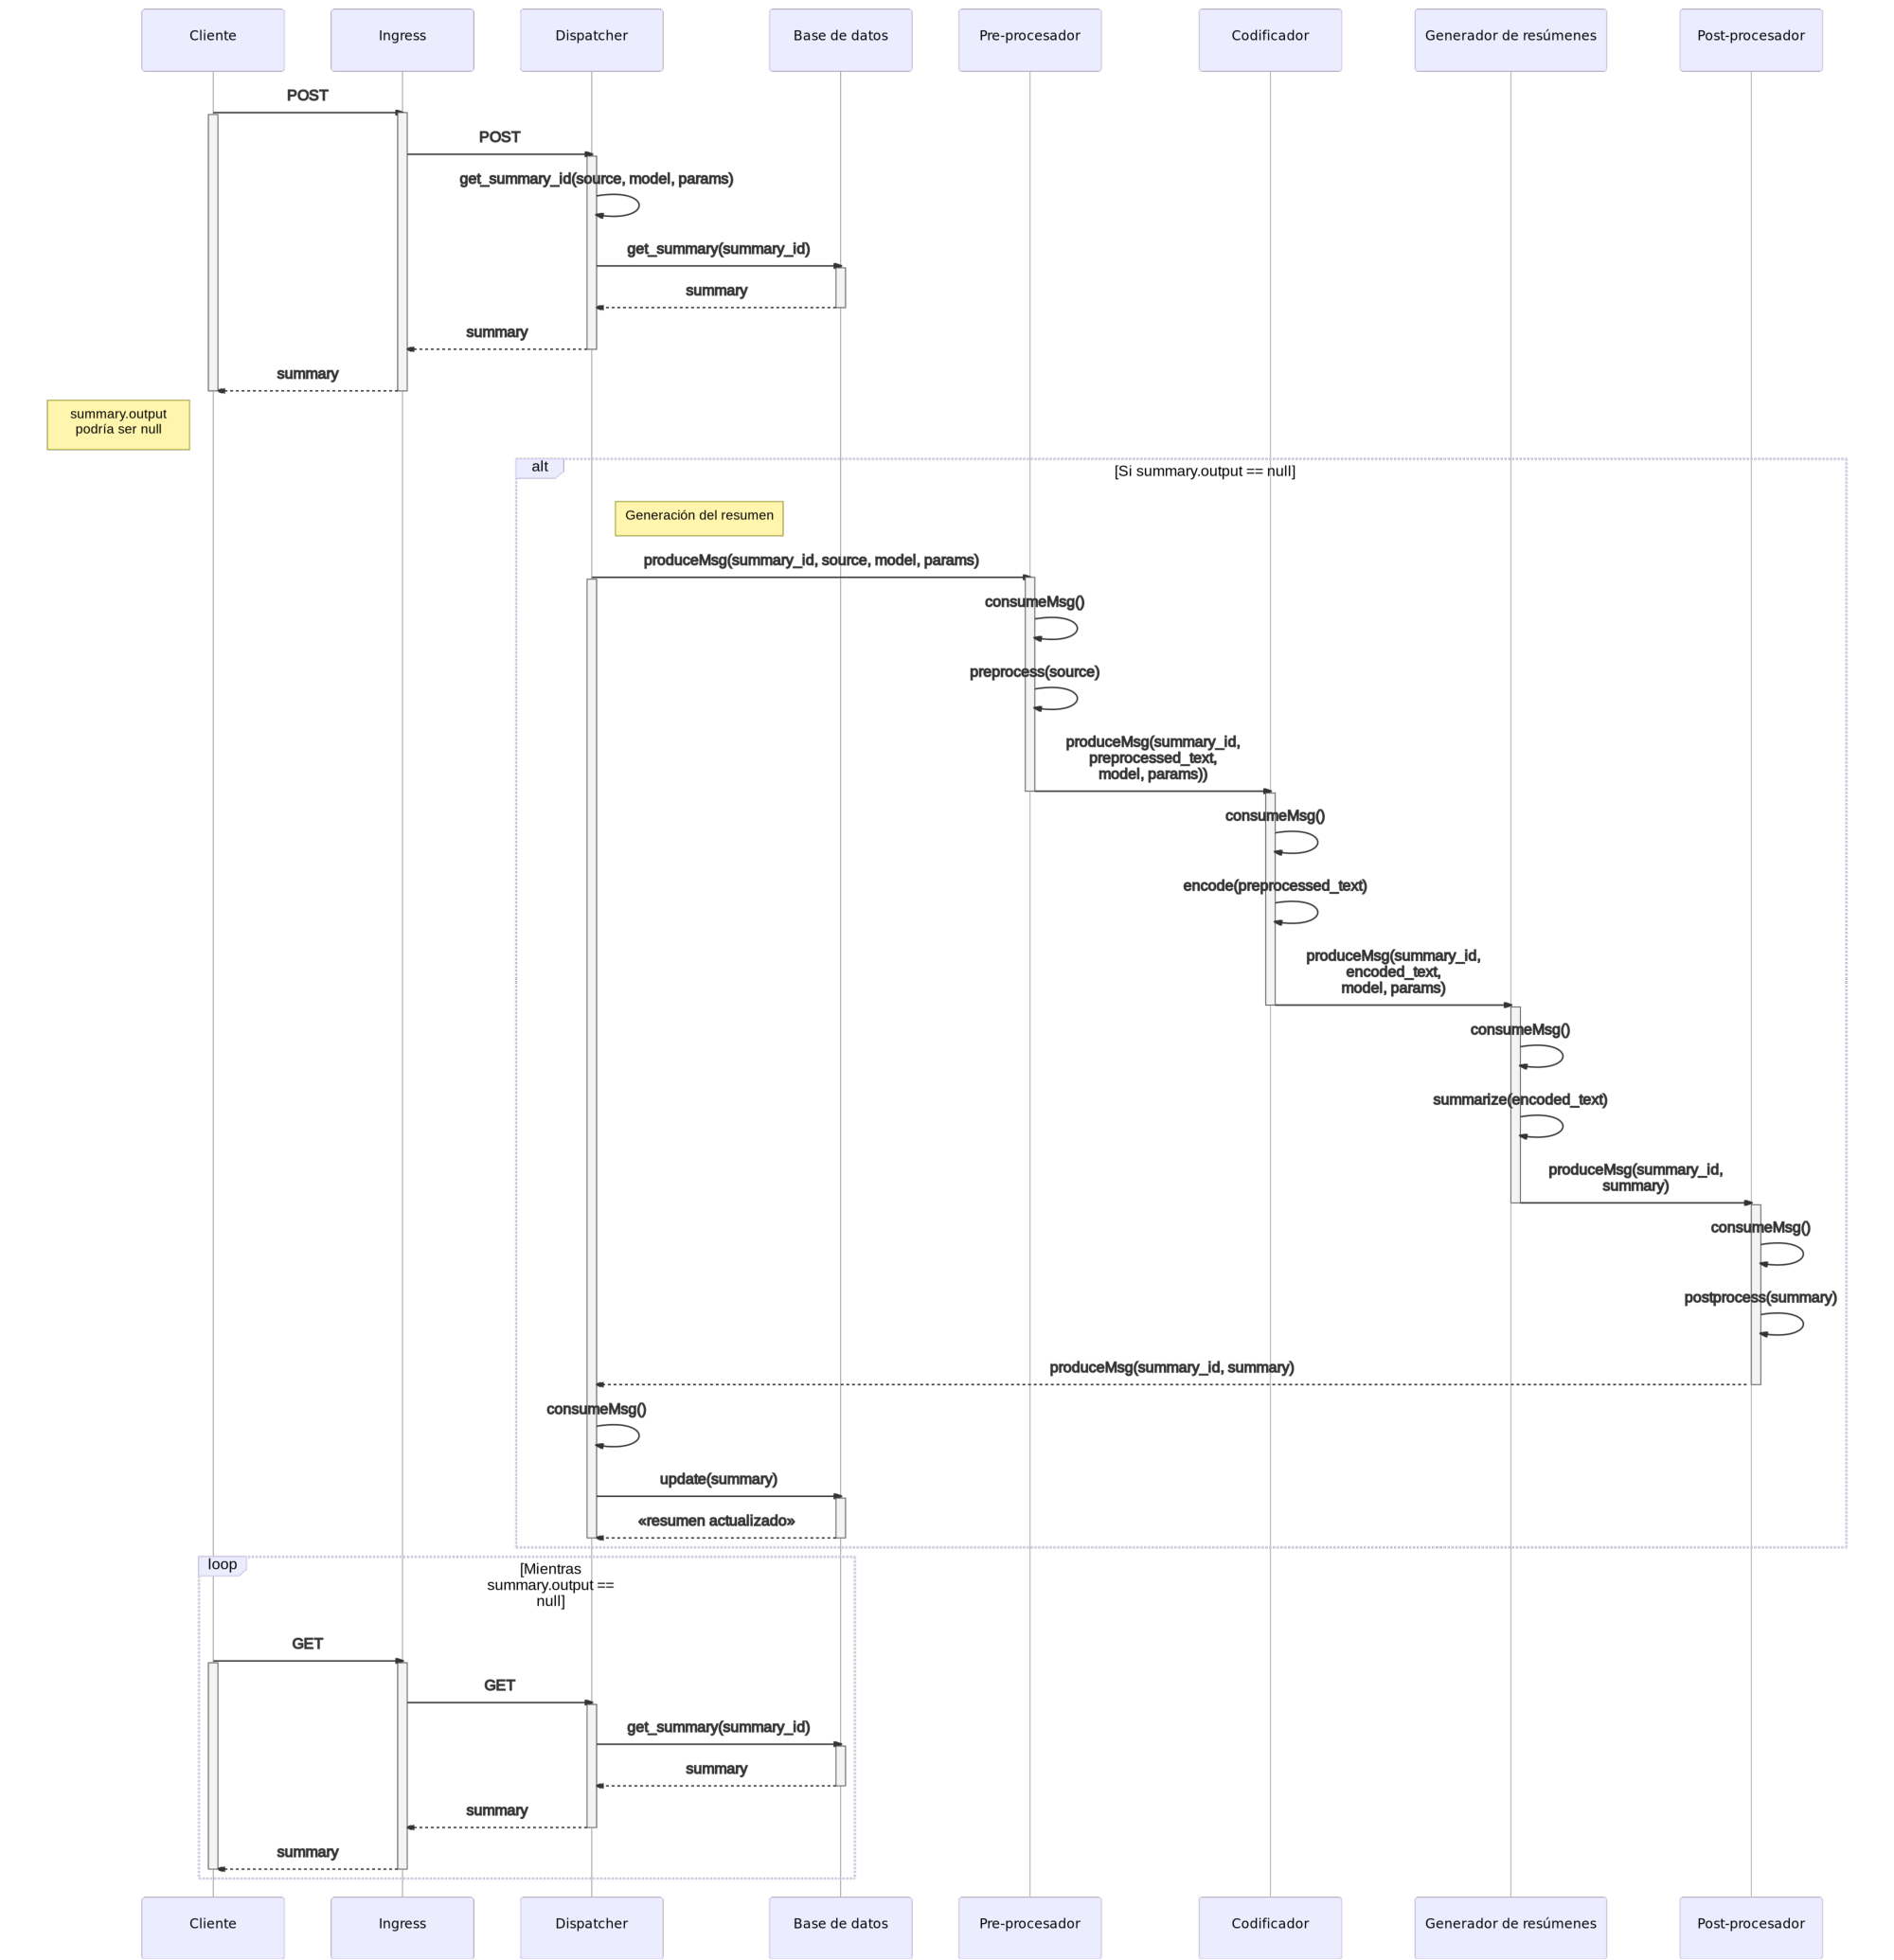
\includegraphics[width=\textwidth]{seq-diagram-api}
	\caption{Diagrama de secuencia del \emph{backend}.}
	\label{seq-api}
\end{figure}

\vspace*{1cm}

\begin{landscape}
	\begin{figure}[h]
		\centering
		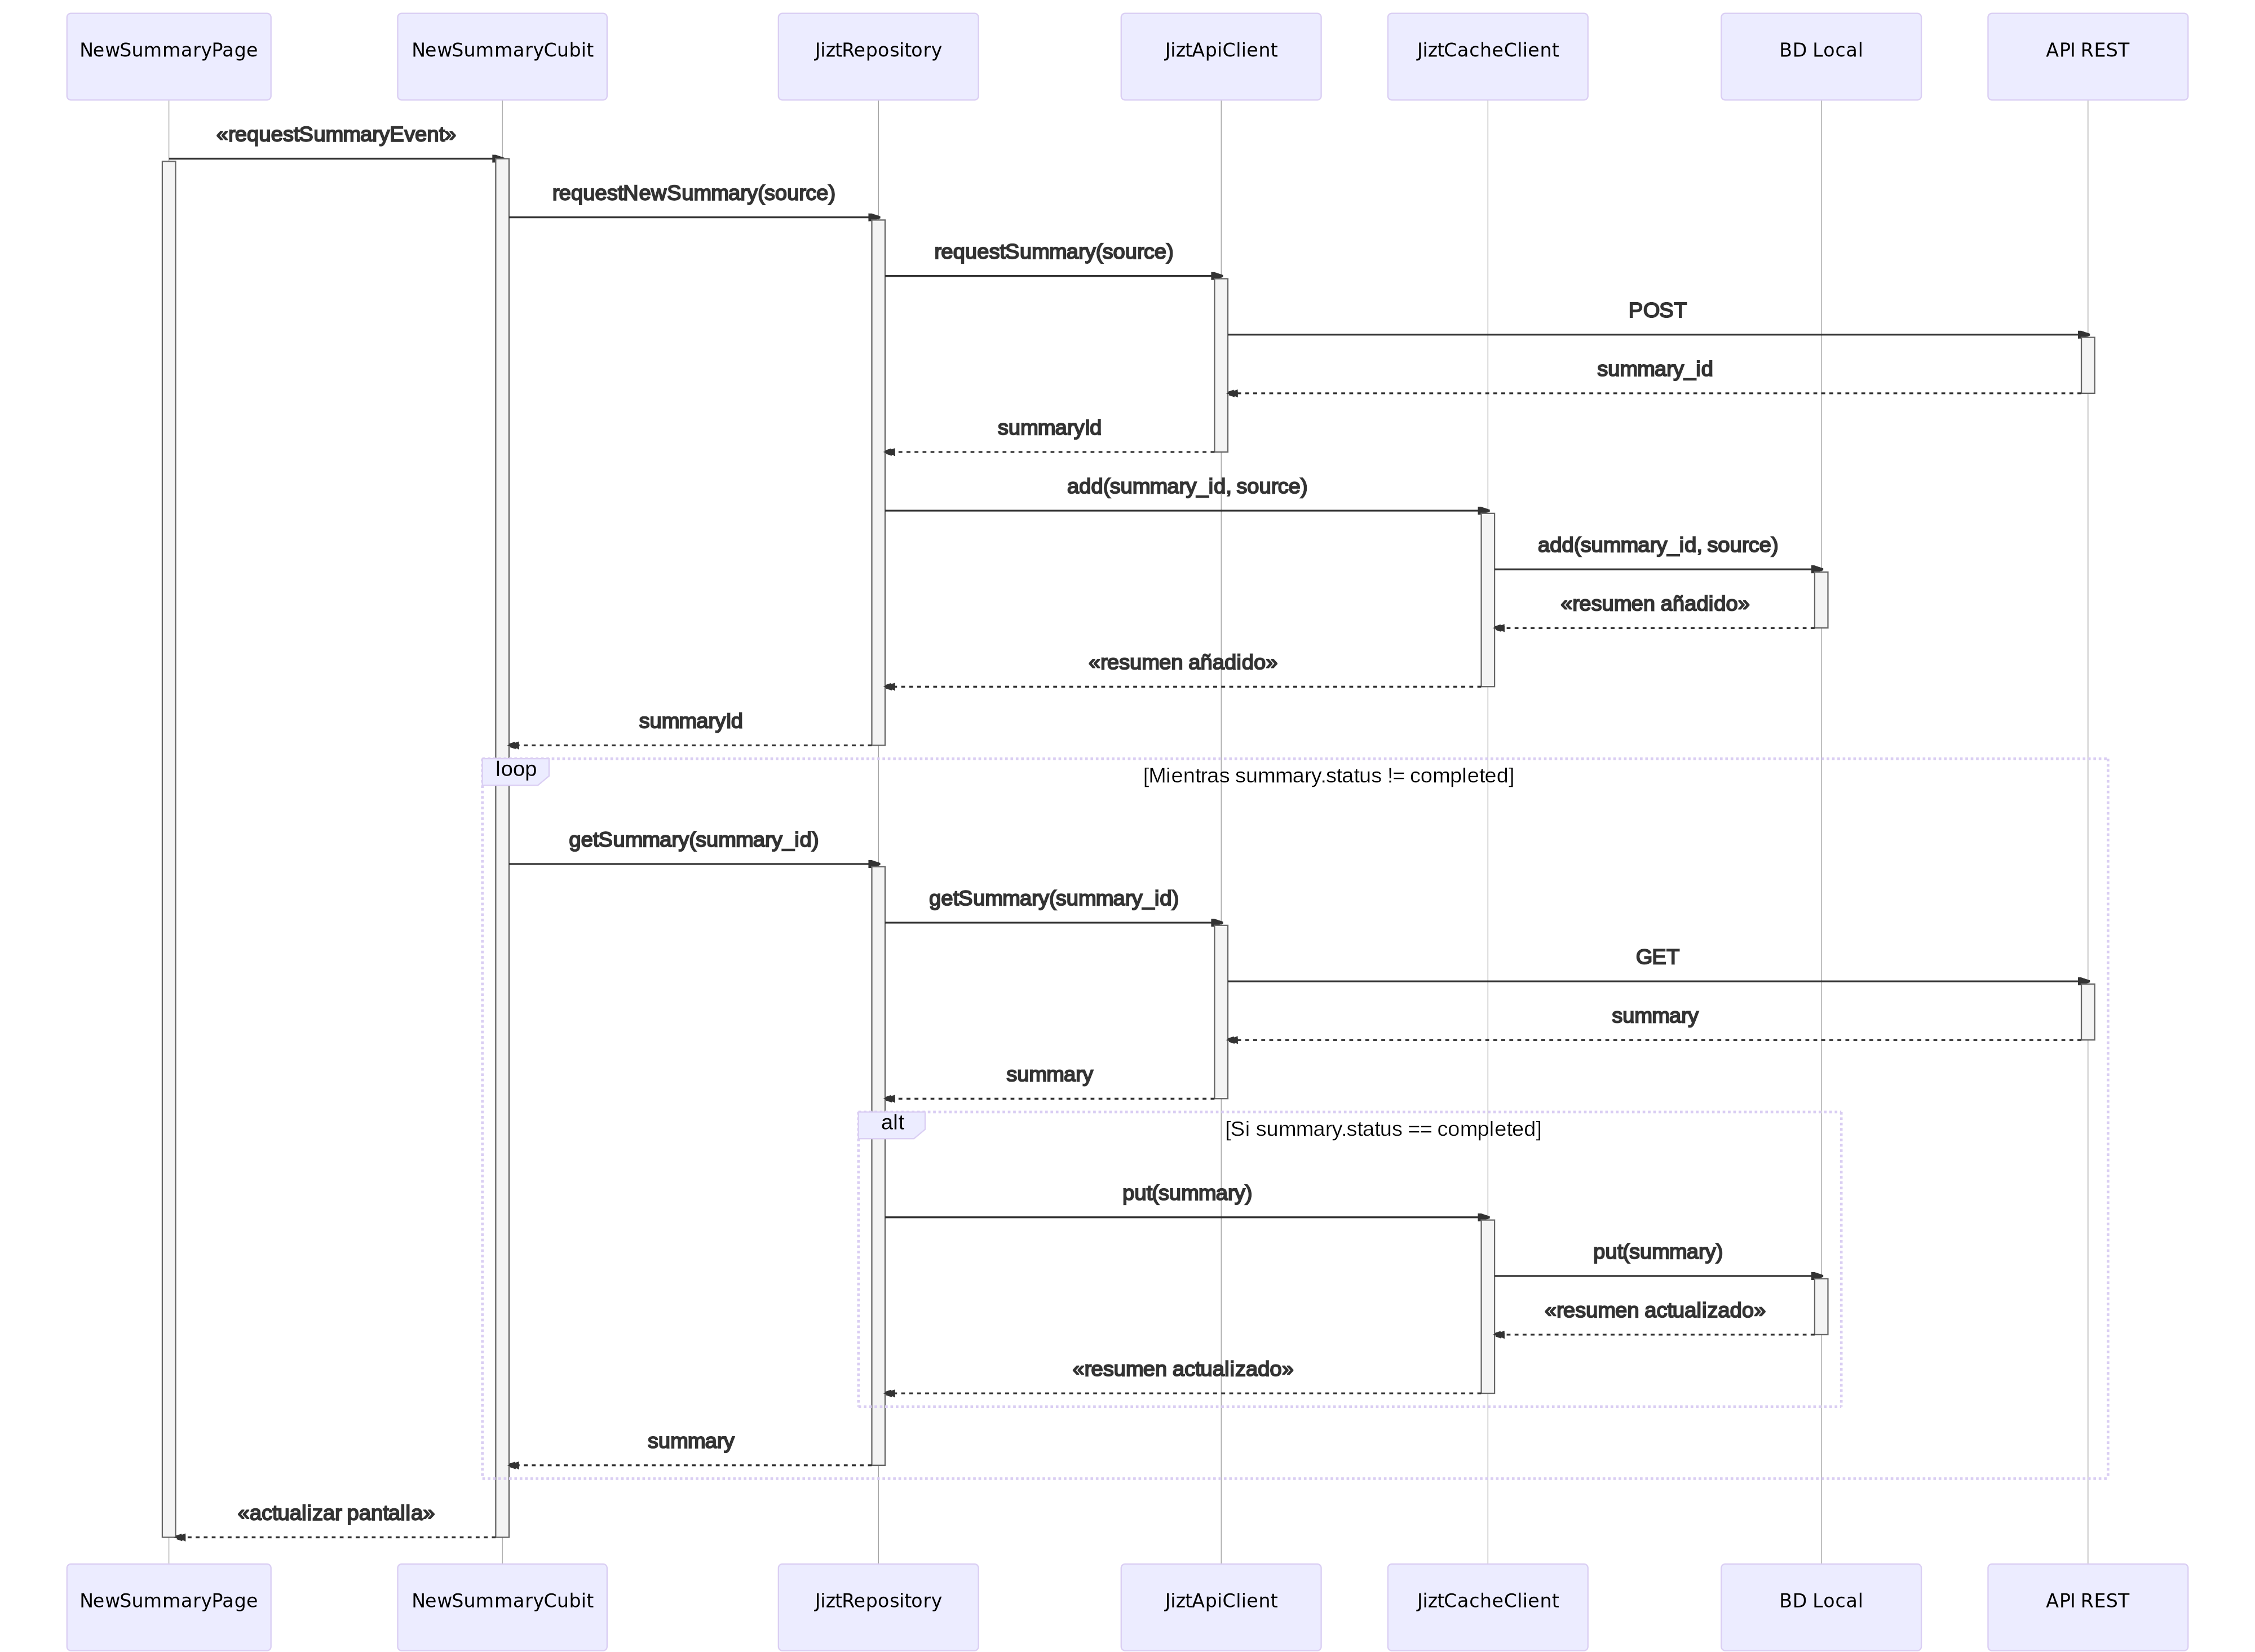
\includegraphics[width=1.3\textwidth]{seq-diagram-app}
		\caption{Diagrama de secuencia de la aplicación.}
		\label{seq-app}
	\end{figure}
\end{landscape}

\section{Diseño arquitectónico}

Dado que el diseño arquitectónico conforma uno de los principales aspectos a destacar de todo el proyecto, se ha incluido de manera detallada en la Memoria.

\subsubsection{\Large \emph{Backend}}

Por tanto, en esta sección llevaremos a cabo un resumen de los principales puntos de la arquitectura, e incluiremos información adicional acerca de los retos que surgieron, y cómo se resolvieron, dando con el diseño arquitectónico final.

Como se indica en la Memoria, para el \emph{backend} se ha desarrollado una \textbf{arquitectura de microservicios}, a través de la cual podemos separar cada paso en la generación de resúmenes (pre-procesado, codificación, generación del resumen, post-procesado0), en módulos independientes, favoreciendo los siguientes aspectos:

\vspace{-0.2cm}
\begin{itemize} [\textbullet]
	\item Gracias a la división en microservicios, conseguimos una gran flexibilidad; los cambios en uno de los pasos en la generación del resumen no influyen al resto.
	
	\item Facilita la detección y corrección de cuellos de botella en el proceso, dado que podemos monitorizar de forma precisa el rendimiento de cada microservicio.
	
	\item La arquitectura es fácilmente escalable tanto en términos de los microservicios ya existentes, aumentando el número de réplicas de cada microservicio (permitiendo la generación en paralelo de varios resúmenes), como en términos de la adicción de nuevos microservicios, por ejemplo, diferentes modelos para distintos idiomas.
	
	\item Asegura una alta disponibilidad, ya si uno de los microservicios falla, el sistema crea una nueva instancia y finaliza el microservicio defectuoso. Adicionalmente, con una arquitectura de microservicios eliminamos cualquier posible punto de único fallo (\emph{single point of failure}).
\end{itemize}

Otro de los principales aspectos de la arquitectura es cómo se lleva a cabo la comunicación y el correcto enrutado de los mensajes entre los diferentes microservicios. Al tratarse de un proceso secuencial, la salido de un microservicio será la entrada del siguiente.

Inicialmente, se pensó en resolver esta situación mediante el patrón de \emph{routing-slips} (hojas de ruta) \cite{routing-slip}. Con este patrón se incluye en el propio mensaje la ruta que este debe seguir, por lo que, implementando un \emph{router} en cada microservicio que interpretara la hoja de ruta, podríamos, resolver el problema del enrutado. En cuanto a cómo se llevaría a cabo la comunicación, esta se podría hacer mediante peticiones HTTP, de forma que cada microservicio implementara su propia REST API.

Siguiendo esta estrategia, junto con el patrón de API \emph{gateway}, a través que se ofrece un punto de entrada al \emph{backend}, el diseño de la arquitectura quedaba como se muestra en la \autoref{fig:deprecated-arch}.

Poco después, conocimos acerca de la \textbf{arquitectura dirigida por eventos} \cite{event-driven}, y de Kafka \cite{apache-kafka}, una de las herramientas más apropiadas y avanzadas a día de hoy para este tipo de arquitectura\footnote{\, De nuevo, referimos al lector a la Memoria, donde se recogen las principales ventajas, tanto de este patrón arquitectónico, como de Kafka.}.

Con este nuevo diseño, la arquitectura se simplificaba en gran medida, y problemas como el escalado, o la entrega fiable de mensajes, corrían a cargo de Kafka, quienes gestionaba estos y otros aspectos de manera automática.

La arquitectura final del \emph{backend} se ilustra en la \autoref{fig:final-arch-backend}.


\subsubsection{\Large \emph{Frontend}}

Gracias a la vibrante comunidad de Flutter \cite{flutter-es}, dar con la arquitectura más apropiada para la aplicación resultó un proceso más fluido.

Antes de comenzar este proyecto, habíamos oído del concepto de \emph{Clean Architecture} \cite{martin15}, aunque no habíamos indagado muy en profundidad en sus proposiciones. No obstante, en nuestra formación de Flutter, apareció de nuevo, e incluso supimos que existe un paquete para Flutter que simplifica la implementación de este patrón \cite{flutter-clean-arch}.

A continuación, nos informamos sobre el patrón BLoC \cite{bloc-pattern}, muy popular también dentro de la comunidad Flutter. Por suerte, también existe un paquete para la implementación de este patrón \cite{bloc-package}.

Finalmente, la arquitectura quedó como se muestra en la \autoref{fig:final-arch-app}.

La información completa acerca de la arquitectura de la aplicación se encuentra, asimismo, en la Memoria.

\newpage

\vspace*{2cm}

\begin{figure}[h!]
	\centering
	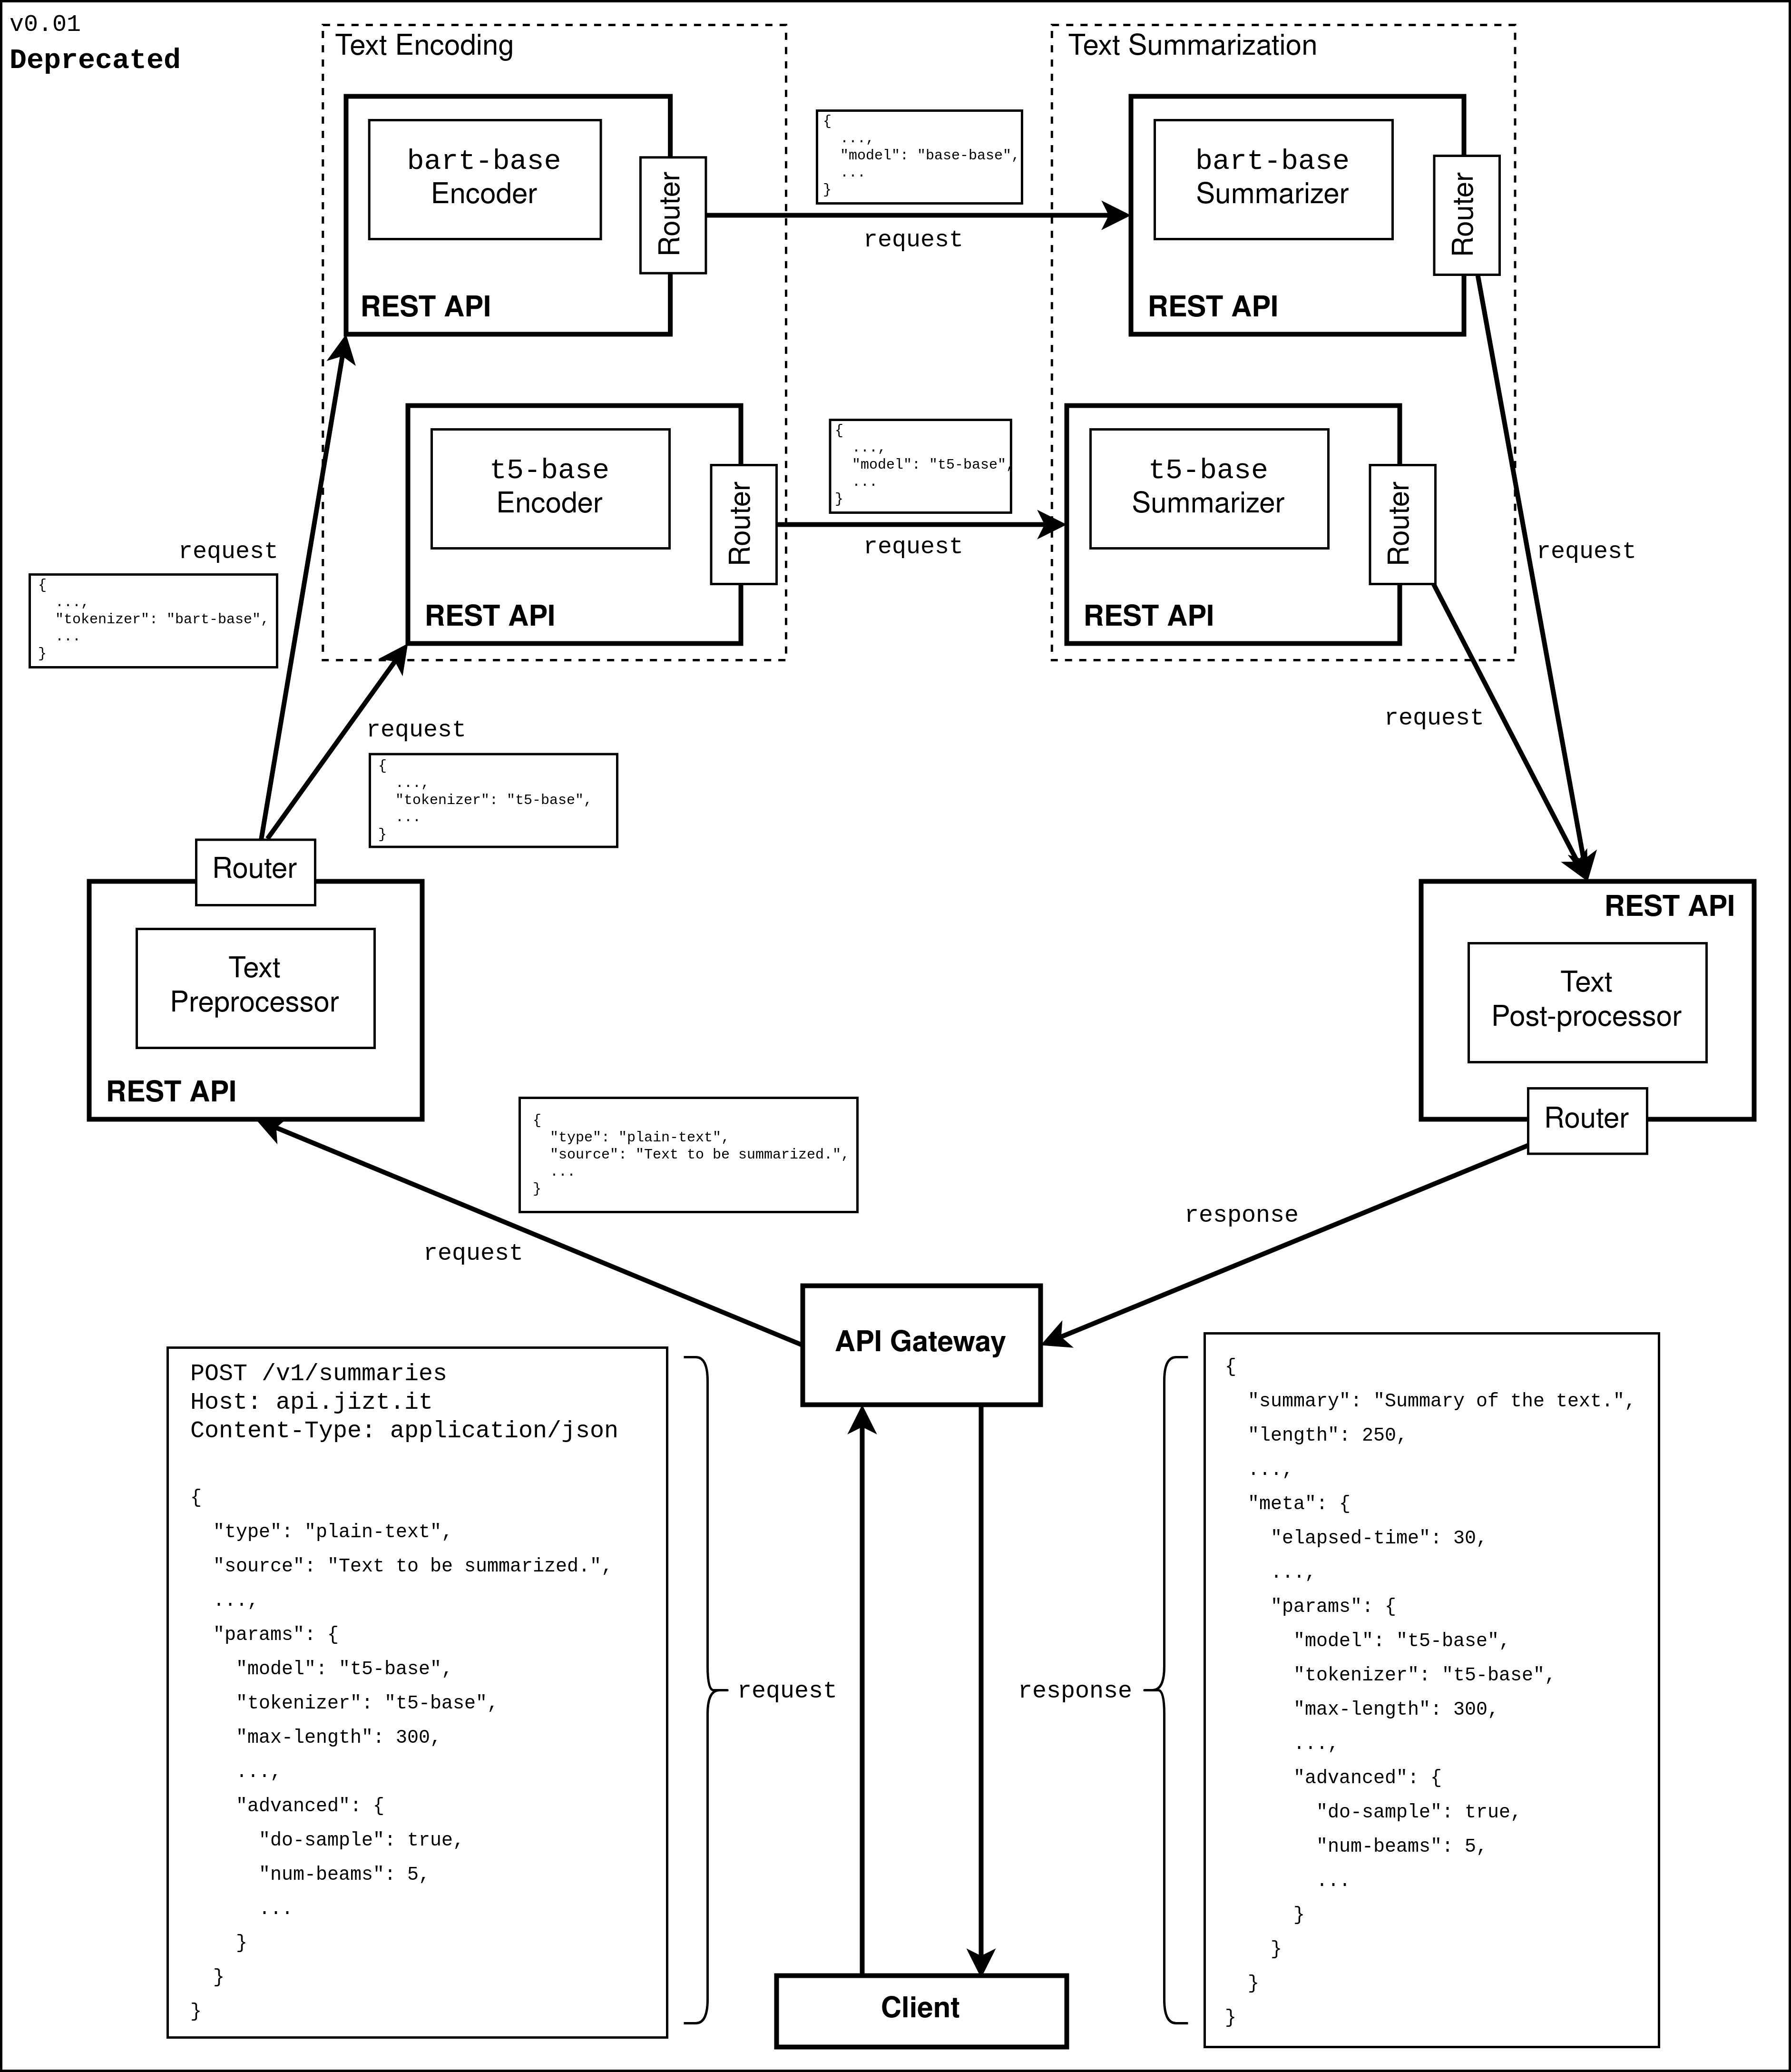
\includegraphics[width=\textwidth]{deprecated-arch}
	\vspace{-0.5cm}
	\caption{Primera aproximación para el diseño arquitectónico del \emph{backend}.}
	\label{fig:deprecated-arch}
\end{figure}

\newpage

\vspace*{2cm}

\begin{figure}[h!]
	\centering
	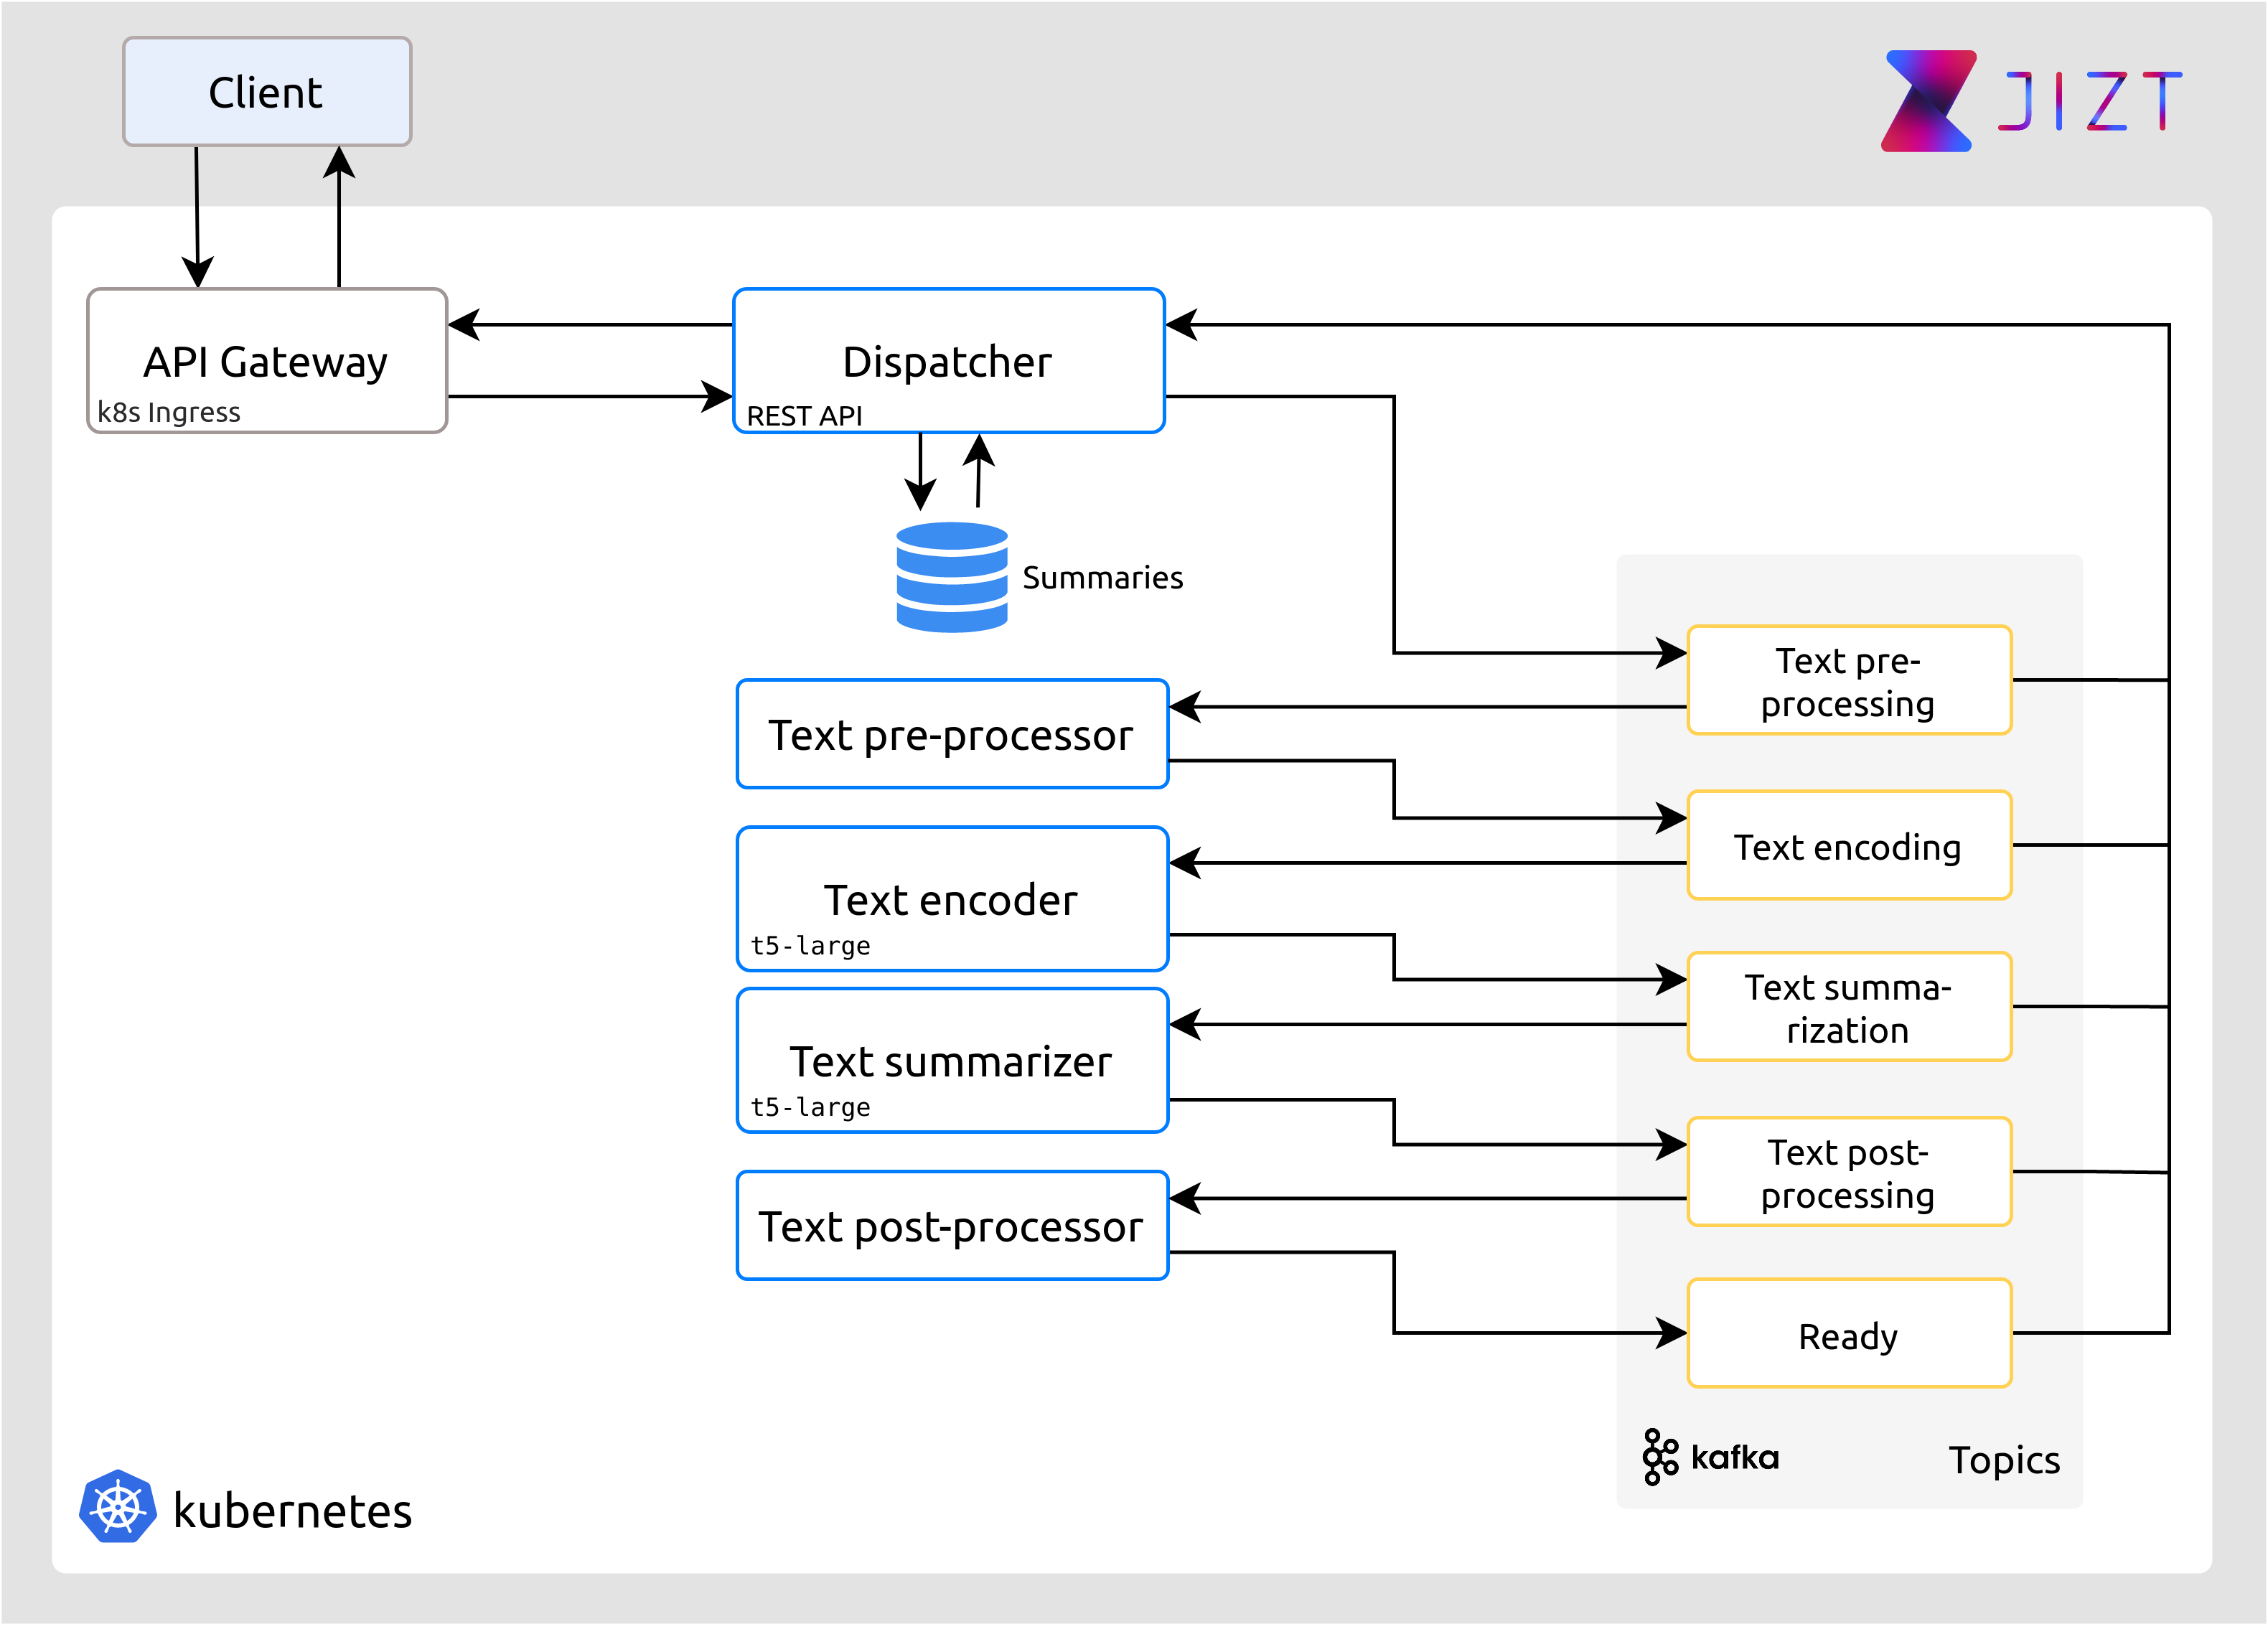
\includegraphics[width=\textwidth]{overview-arch}
	\vspace{-0.5cm}
	\caption{Diseño final de la arquitectura del \emph{backend}.}
	\label{fig:final-arch-backend}
\end{figure}

\begin{figure}[h!]
	\centering
	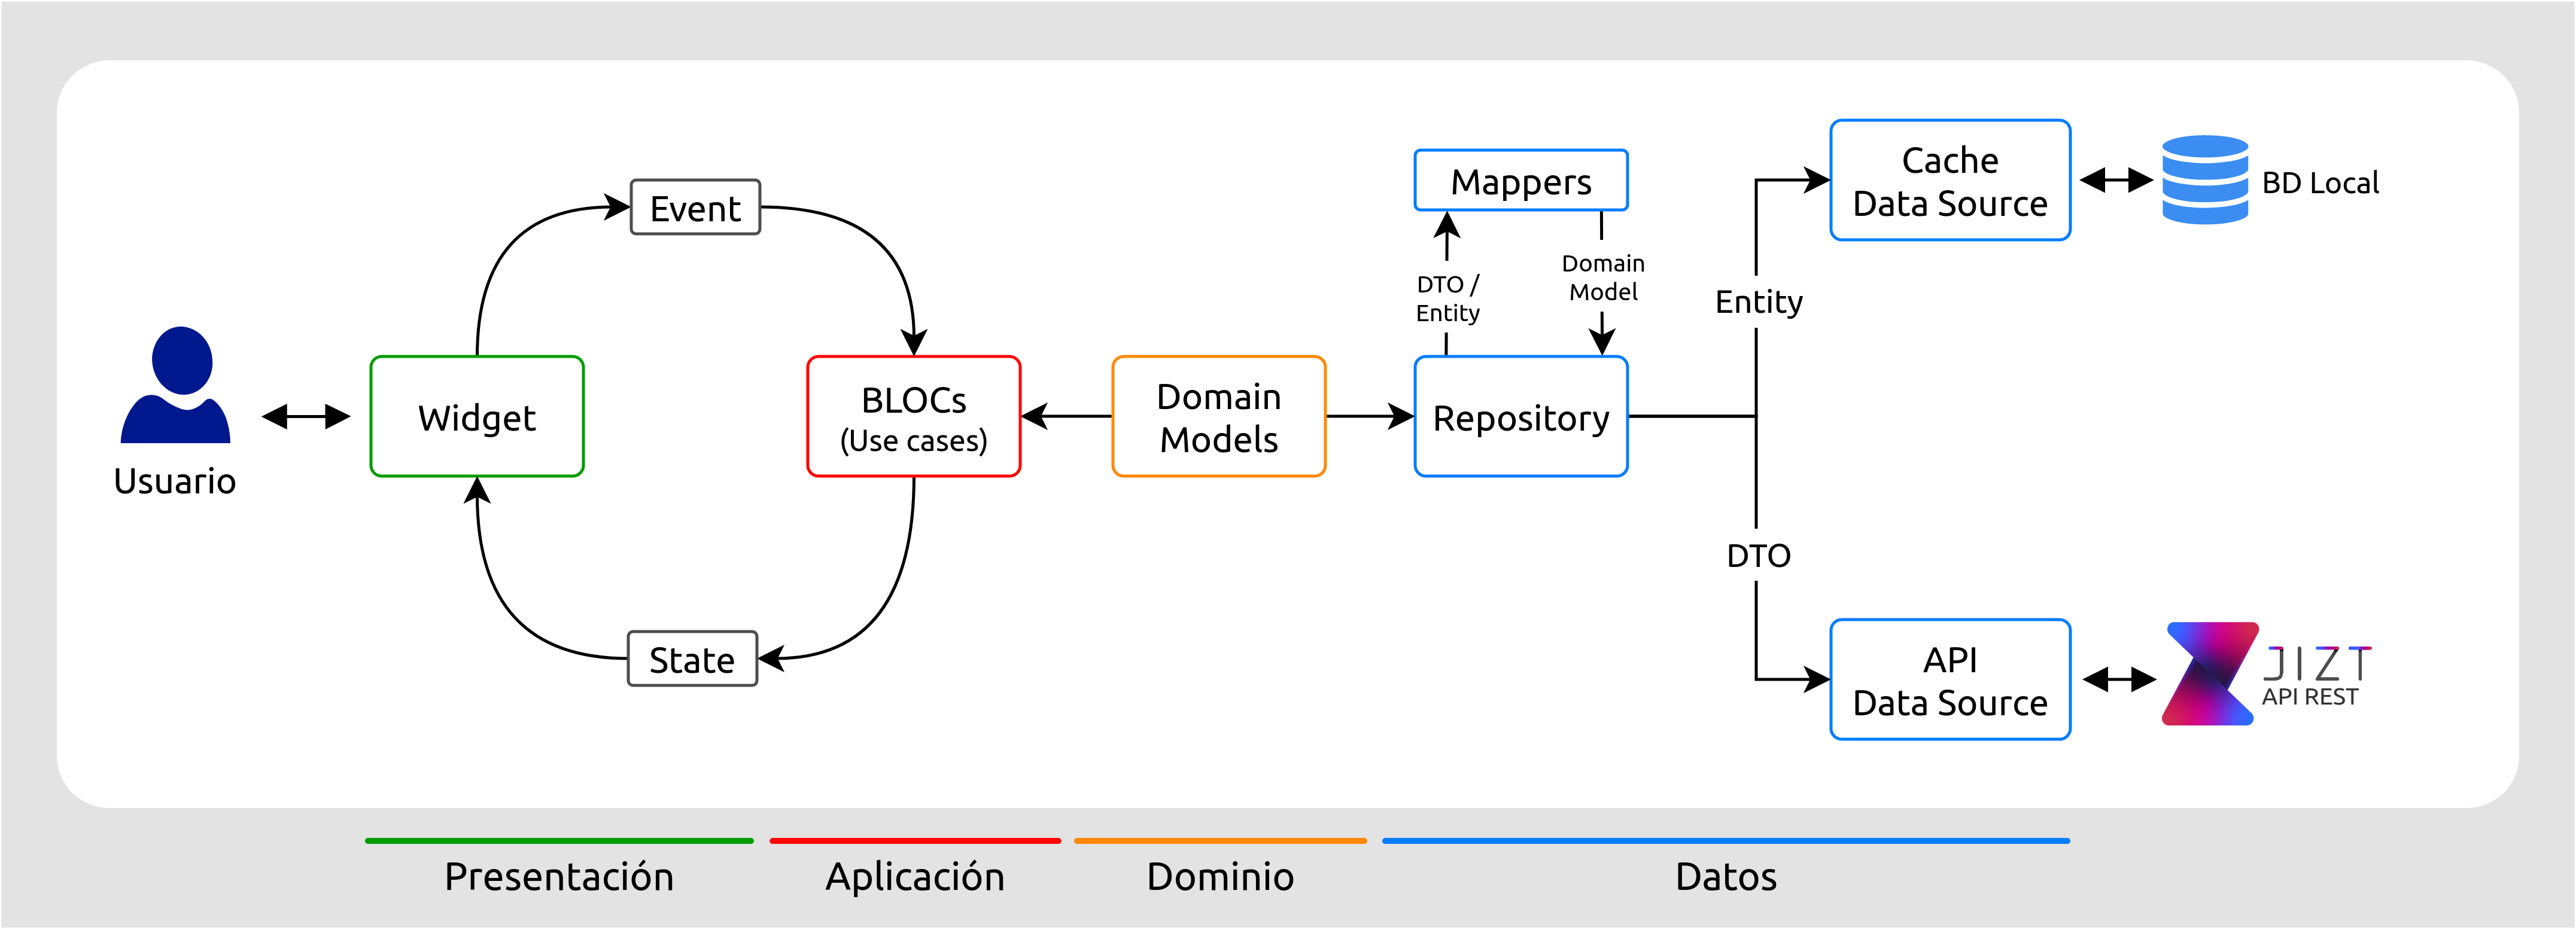
\includegraphics[width=\textwidth]{jizt-app-arch}
	\vspace{-0.5cm}
	\caption{Diseño final de la arquitectura de la aplicación.}
	\label{fig:final-arch-app}
\end{figure}

\newpage

\section{Diseño de interfaces}

\subsubsection{Diseño del logo}

Una de las intenciones detrás de este proyecto siempre ha sido tratar de crear una cierta imagen corporativa y de producto. Como consecuencia, el diseño de nuestra carta de presentación, es decir, nuestro logo, ocupó un papel central en las primeras iteraciones del proyecto.

En la búsqueda creativa de un logo atractivo, moderno y memorable, se experimentó con numerosos posibles diseños en papel.

\begin{figure}[h!]
	\centering
	\includegraphics[width=\textwidth]{logo-drafts}
	\vspace{-0.5cm}
	\caption{Ideas, ideas, y más ideas. Pero solo unas pocas buenas.}
\end{figure}

Finalmente, dimos con un diseño que parecía tener potencial. Cogimos nuestro ordenador, y nos sumergimos en Adobe Illustrator, un editor de gráficos vectoriales muy popular. Por experiencia previa en diseño gráfico (autodidacta), sabemos que, teniendo una buena idea de partida, equivale a tener una gran parte del trabajo hecho.

Así pues, el logo final, nuestra carta de presentación, acabó luciendo como se muestra en la \autoref{fig:jizt-logo}. En nuestra opinión, cumple con los requisitos esperados.

\newpage

\begin{figure}[h!]
	\centering
	
\includegraphics[width=0.8\textwidth]{jizt-logo}
	\caption{JIZT - Generación de resúmenes mediante IA.}
	\label{fig:jizt-logo}
\end{figure}

\vspace{0.3cm}

\begin{figure}[H]
	\centering
	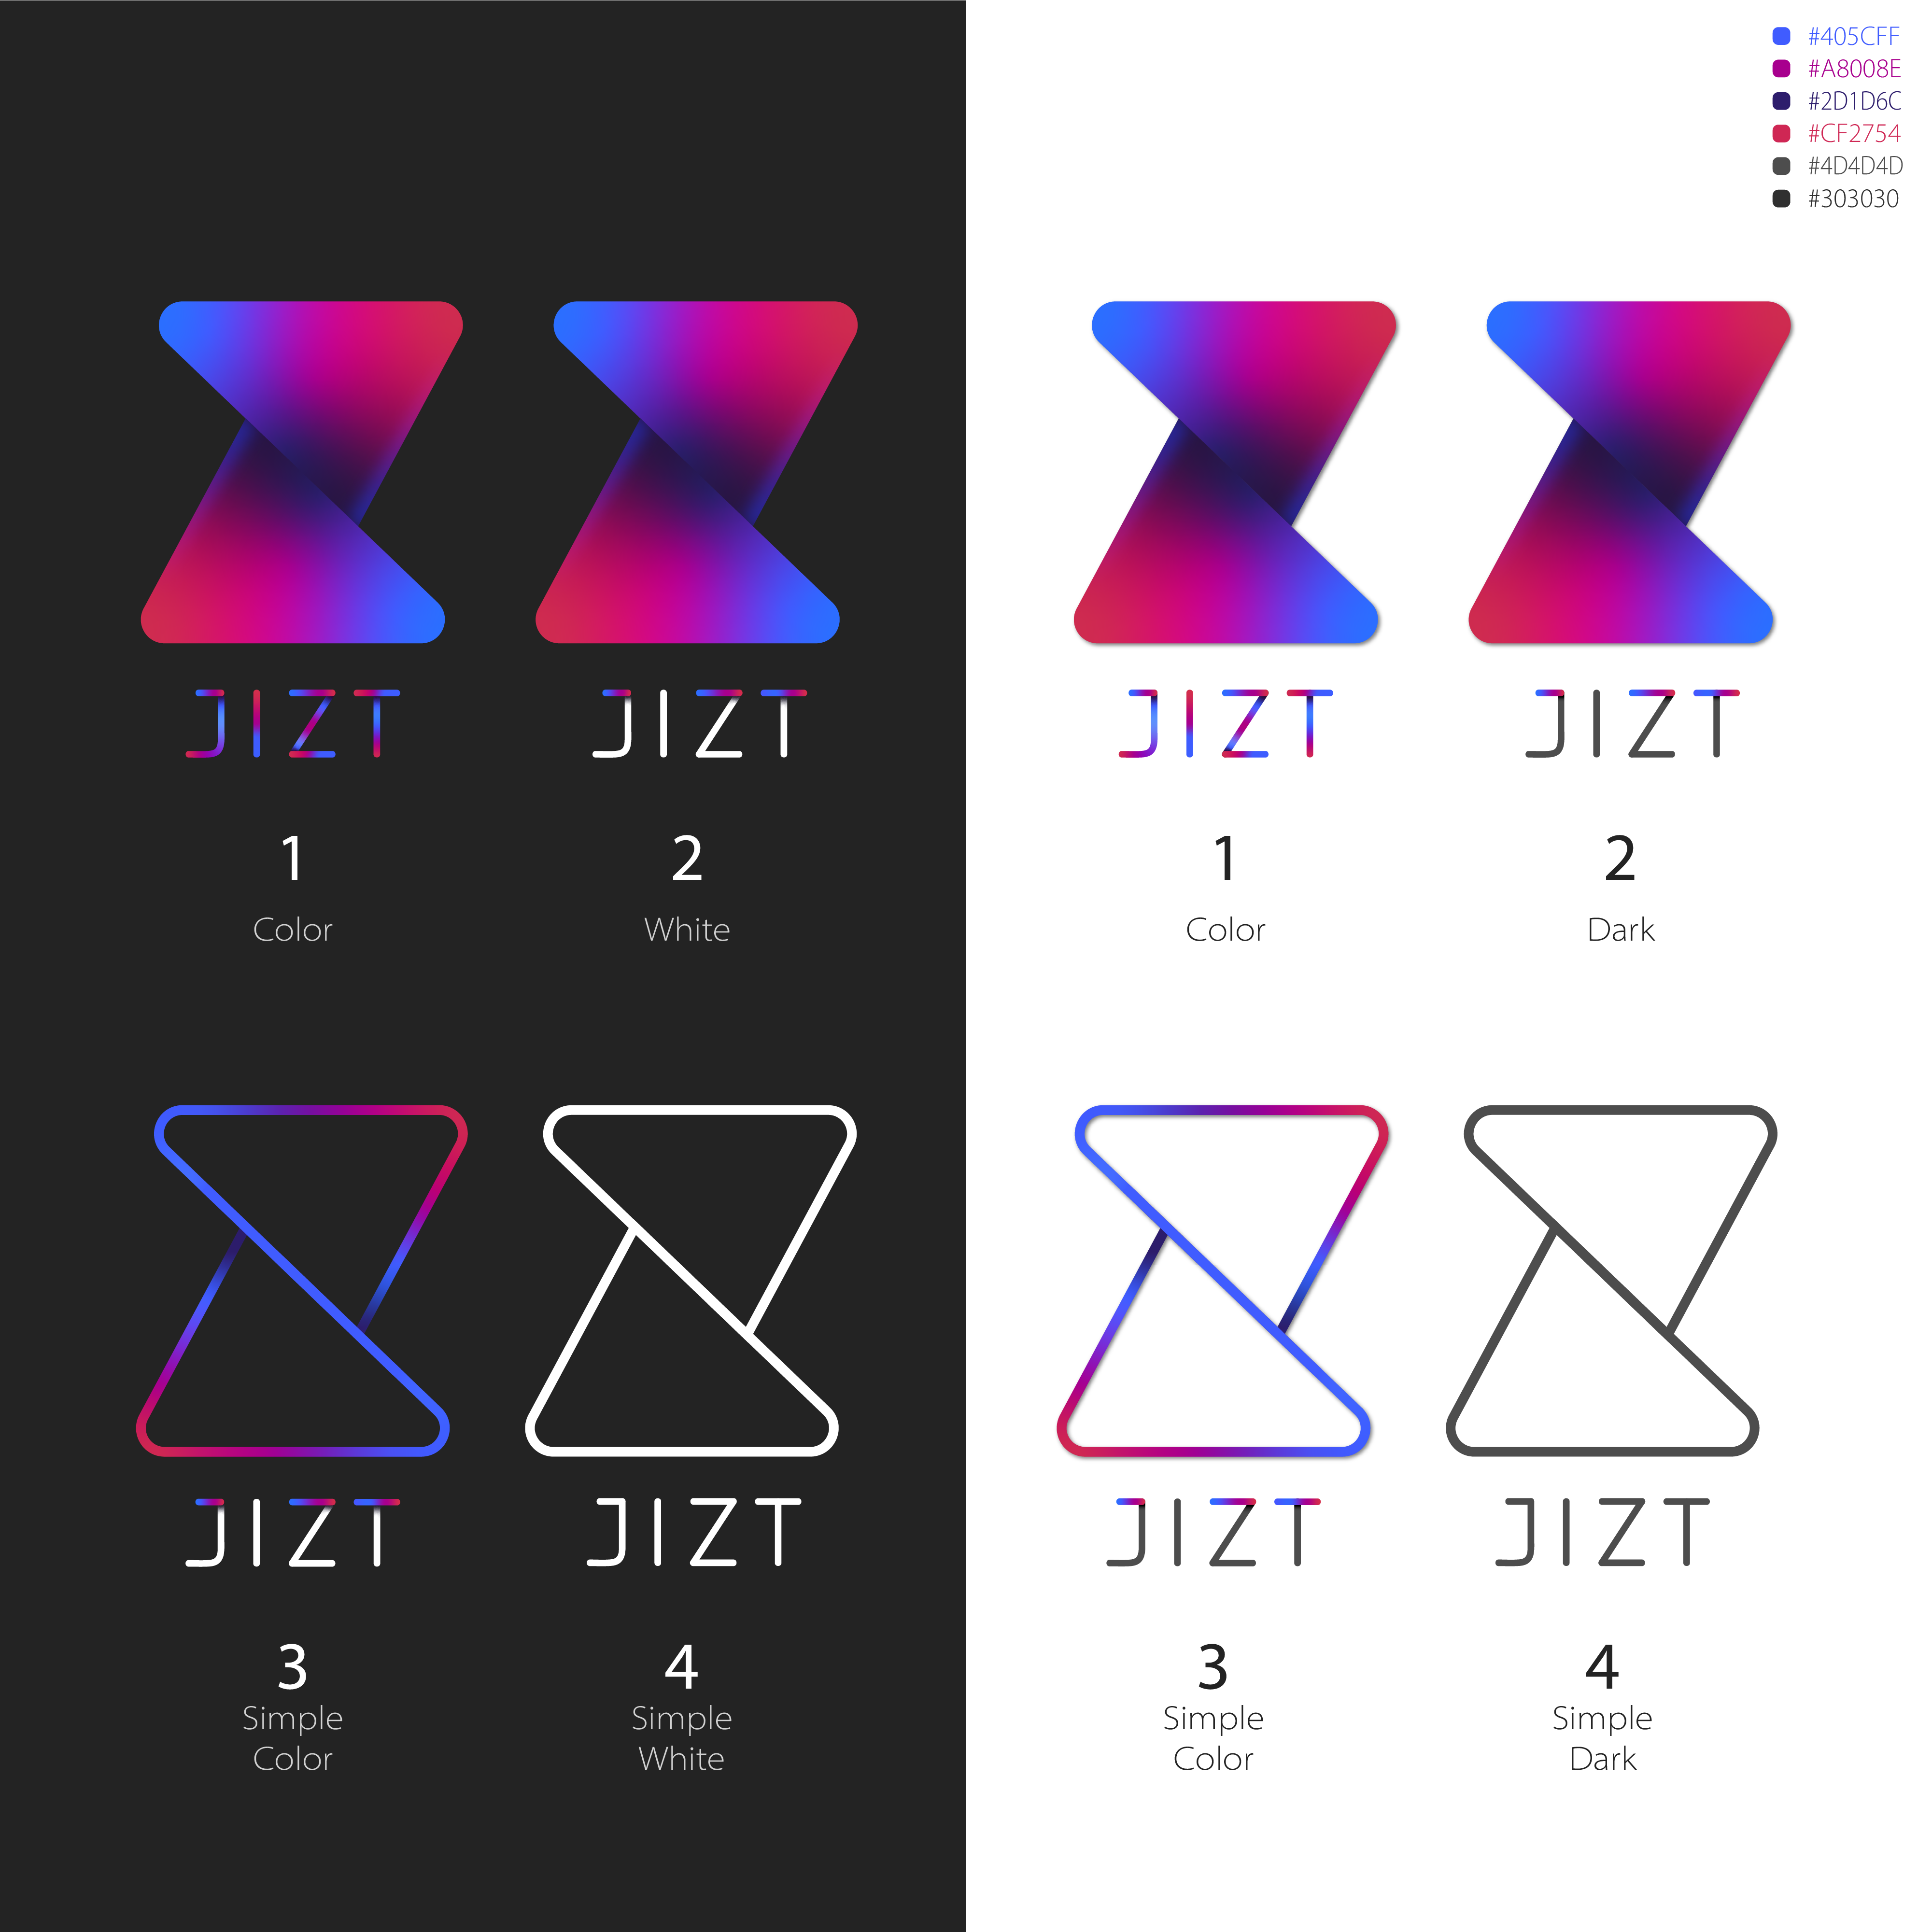
\includegraphics[width=0.91\textwidth]{jizt-logo-variations}
	\caption{Variaciones sobre el logo de JIZT.}
\end{figure}

\newpage

\subsubsection{Diseño de la interfaz gráfica de la aplicación}

Para el diseño de la interfaz gráfica de usuario de la aplicación, trabajamos directamente sobre el ordenador, esta vez con el programa Inkscape, también editor de gráficos vectoriales, pero en este caso \emph{open-source} y gratuito.

Se llevaron a cabo diferentes iteraciones hasta dar con un diseño que nos acabó pareciendo adecuado.

\bigskip

\begin{figure}[h!]
	\centering
	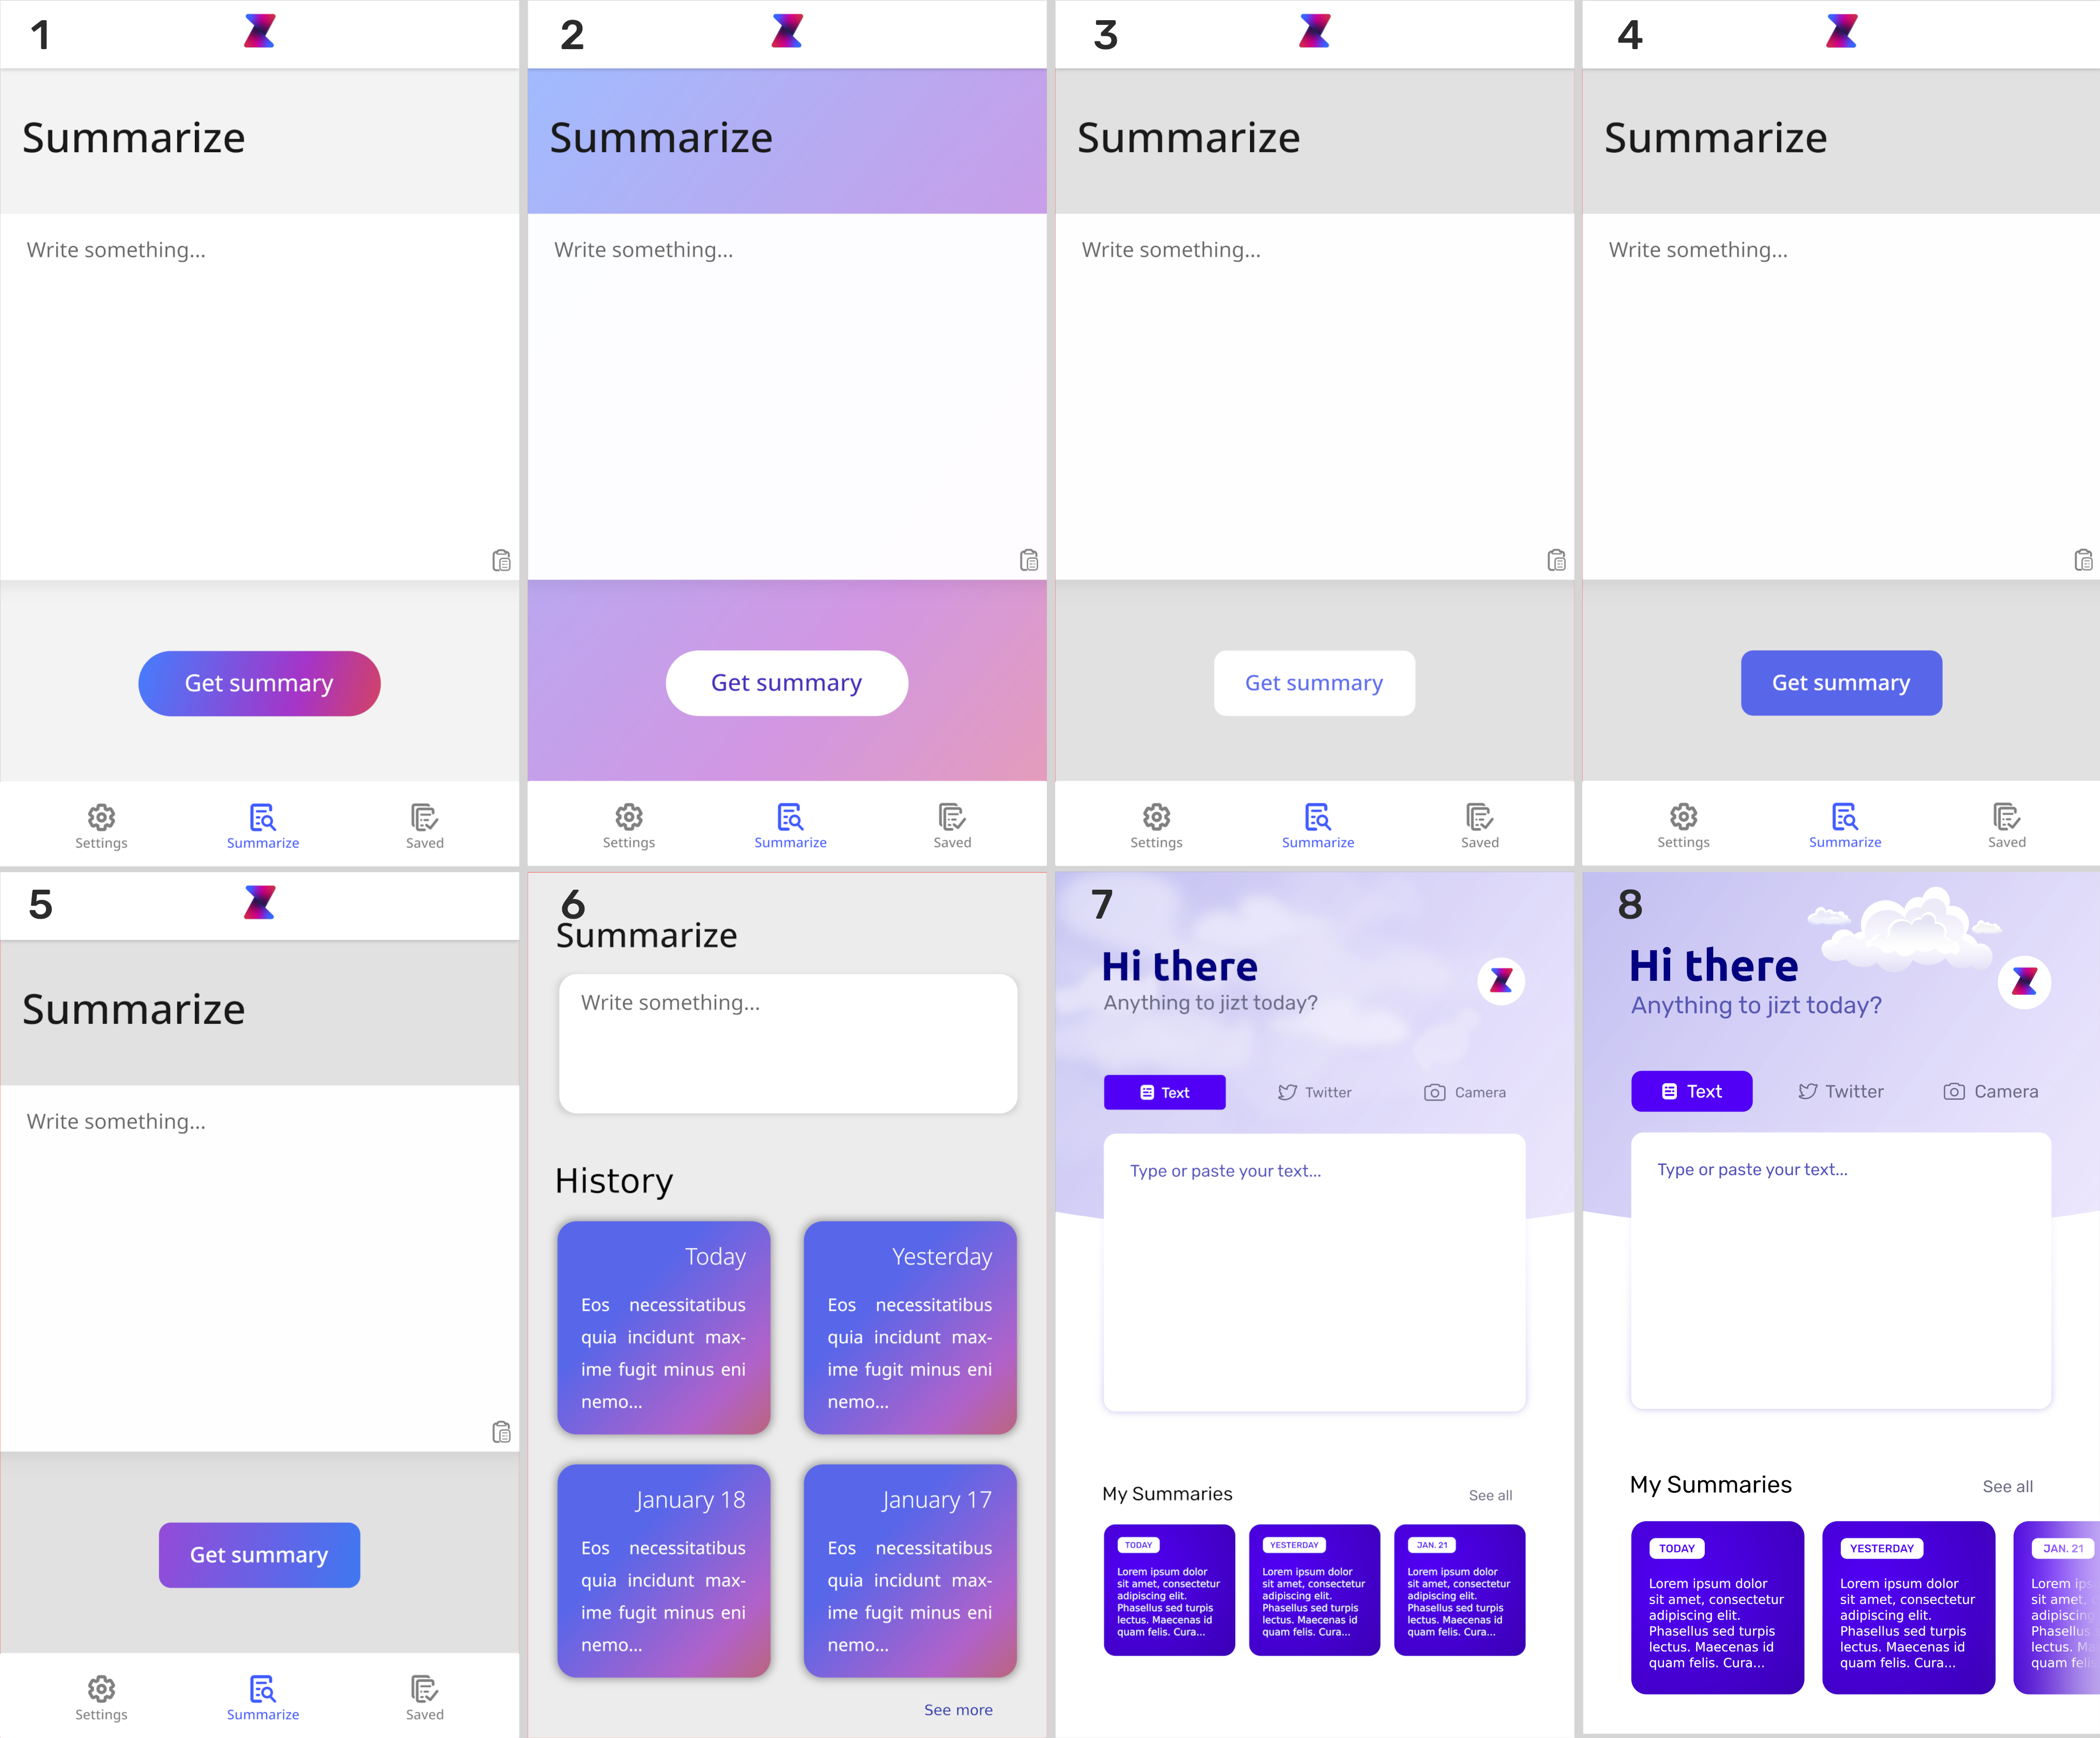
\includegraphics[width=\textwidth]{ui-design}
	\vspace{-0.5cm}
	\caption{Iteraciones sobre la pantalla principal.}
\end{figure}

Siguiendo el estilo de la pantalla principal, se diseñaron el resto de pantallas, las cuales se muestran en la \autoref{fig:app-screens}.

\newpage

\vspace*{1cm}
\begin{figure}[h!]
	\centering
	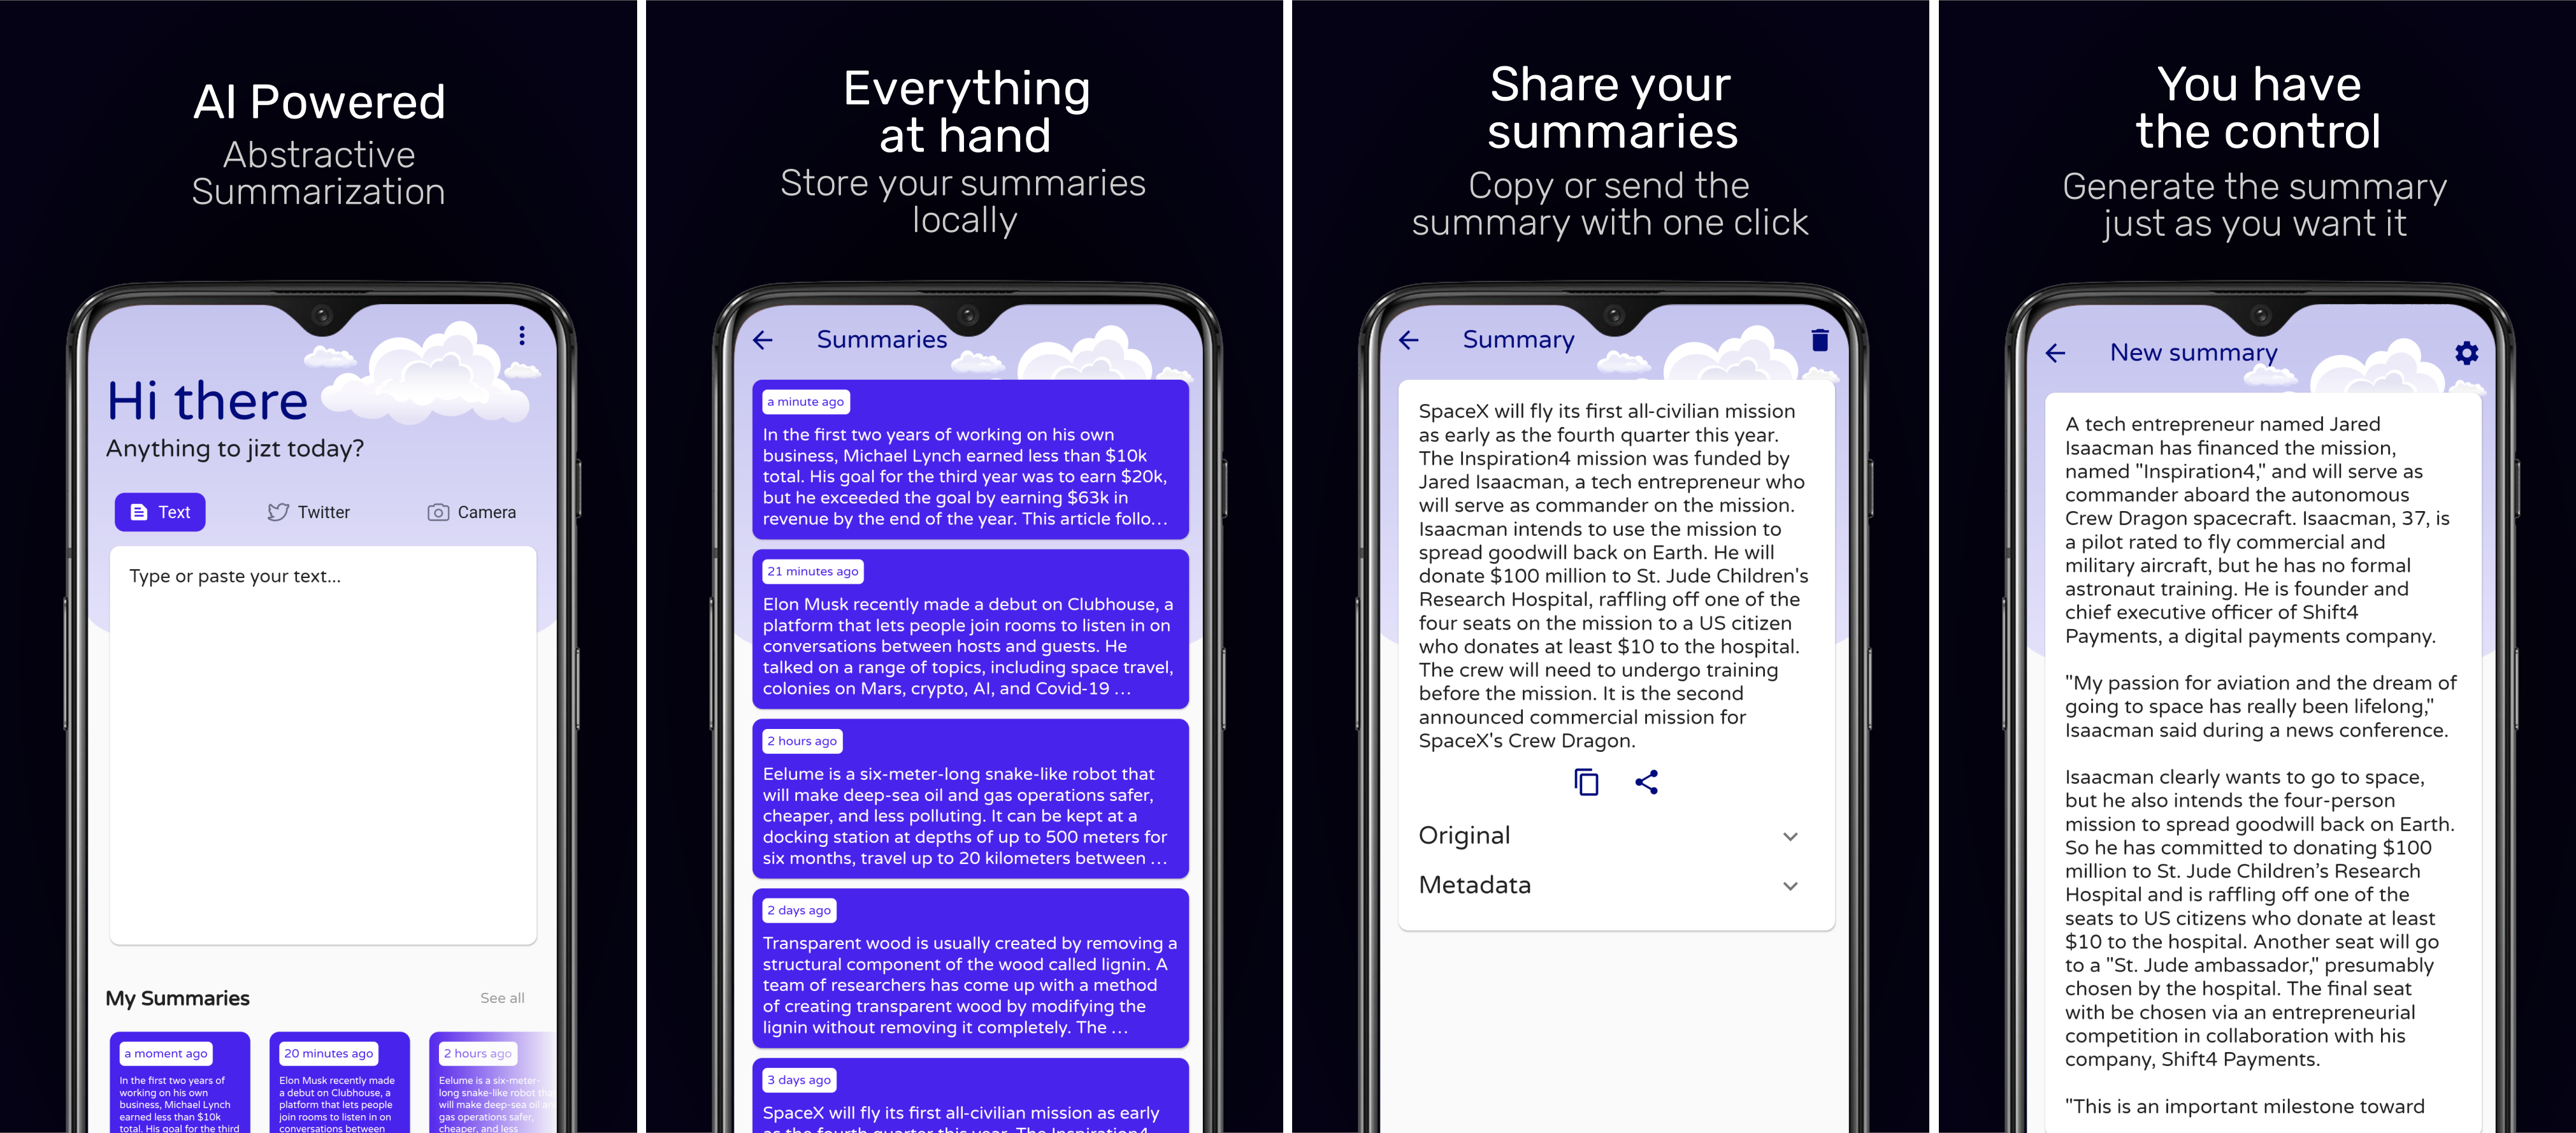
\includegraphics[width=\textwidth]{app-screens}
	\vspace{-0.5cm}
	\caption{Capturas de pantalla de la aplicación para su publicación en Play Store.}
    \label{fig:app-screens}
\end{figure}
